\documentclass[12pt,a4paper]{report}

% Page Geometry & Margins
\usepackage[top=1in,bottom=1in,left=1.2in,right=1in]{geometry}

% Core Packages
\usepackage[utf8]{inputenc}
\usepackage[T1]{fontenc}
\usepackage{amsmath,amssymb}
\usepackage{fouriernc}
\usepackage[dvipsnames,svgnames,x11names]{xcolor}
\colorlet{indigo}{blue!70!black}
\colorlet{teal}{green!50!blue}
\colorlet{amber}{orange!80!yellow}
\usepackage{graphicx}
\usepackage{booktabs}
\usepackage{setspace}
\usepackage{caption}
\usepackage{titlesec}
\usepackage{fancyhdr}
\usepackage[protrusion=true,expansion=false]{microtype}
\usepackage{tabularx}

% Algorithms
\usepackage{algorithm}
\usepackage{algpseudocode}

% TikZ for Diagrams
\usepackage{tikz}
\usetikzlibrary{shapes.geometric, arrows.meta, positioning, calc, backgrounds}

% Hyperref Setup
\usepackage[hidelinks]{hyperref}

% Line Spacing
\setstretch{1.2}

% Header and Footer setup
\pagestyle{fancy}
\fancyhf{}
\fancyhead[R]{\small\slshape\leftmark}
\fancyfoot[C]{\thepage}
\renewcommand{\headrulewidth}{0.4pt}
\setlength{\headheight}{15pt}

% Title formats
\titleformat{\chapter}[display]
  {\normalfont\huge\bfseries}{\chaptertitlename\ \thechapter}{18pt}{\Huge}
\titlespacing*{\chapter}{0pt}{10pt}{25pt}

% Front matter TOC layout (matching ref/main.pdf with bold headings)
\makeatletter
\newcommand{\l@frontmatter}[2]{%
  \vskip 0.6em \noindent {\bfseries #1}\hfill {\bfseries #2}\par
}
\makeatother

\begin{document}

% ==========================================
% COVER / TITLE PAGE
% ==========================================
\begin{titlepage}
\centering
\vspace*{1.0cm}

{\LARGE \textbf{CodeInsight: Automated Codebase Health \&\\[0.3cm] Technical Debt Prioritization Platform}\par}

\vspace{1.0cm}
{\large A report submitted for the course named Project II (CS3202)\par}

\vspace{2.2cm}
{\large Submitted By\par}
\vspace{0.2cm}
{\large \textbf{KRISHNA ANAND}\par}
{\large SEMESTER VI\par}
{\large 230101082\par}

\vspace{1.6cm}
{\large Supervised By\par}
\vspace{0.2cm}
{\large \textbf{DR. RAJKUMARI BIDYALAKSHMI DEVI}\par}

\vspace{2.0cm}

\includegraphics[width=3.2cm]{iiit manipur.png}\par

\vspace{1.0cm}
{\small \textbf{DEPARTMENT OF COMPUTER SCIENCE AND ENGINEERING}\par}
{\small \textbf{INDIAN INSTITUTE OF INFORMATION TECHNOLOGY SENAPATI,}\par}
{\small \textbf{MANIPUR}\par}
\vspace{0.2cm}
{\small \textbf{APRIL 2026}\par}

\end{titlepage}

% ==========================================
% FRONT MATTER (Declaration to List of Tables)
% ==========================================
\pagenumbering{arabic}
\setcounter{page}{1}

% ------------------------------------------
% DECLARATION
% ------------------------------------------
\newpage
\thispagestyle{plain}
\phantomsection
\addcontentsline{toc}{frontmatter}{Declaration}
\begin{center}
    {\LARGE \textbf{Declaration}\par}
\end{center}
\vspace{1.5cm}

In this submission, I have expressed my idea in my own words, and I have adequately cited and referenced any ideas or words that were taken from another source. I also declare that I adhere to all principles of academic honesty and integrity and that I have not misrepresented or falsified any ideas, data, facts, or sources in this submission. If any violation of the above is made, I understand that the institute may take disciplinary action. Such a violation may also engender disciplinary action from the sources which were not properly cited or permission not taken when needed.

\vspace{3.5cm}
\begin{flushright}
\textbf{KRISHNA ANAND}\\
230101082
\end{flushright}

\vspace{1.5cm}
\noindent \textbf{DATE:}

% ------------------------------------------
% CERTIFICATE / TO WHOM IT MAY CONCERN
% ------------------------------------------
\newpage
\thispagestyle{plain}
\phantomsection
\addcontentsline{toc}{frontmatter}{Certificate}

\begin{minipage}[c]{0.18\textwidth}
    
\includegraphics[width=2.2cm]{iiit manipur.png}
\end{minipage}
\begin{minipage}[c]{0.80\textwidth}
    \centering
    {\small \textbf{Department of Computer Science and Engineering}\par}
    {\small \textbf{Indian Institute of Information Technology Senapati, Manipur}\par}
\end{minipage}

\vspace{0.2cm}
\noindent\rule{\textwidth}{0.8pt}

\vspace{0.2cm}
\noindent
\begin{minipage}[t]{0.5\textwidth}
    \small
    \textbf{Dr. Rajkumari Bidyalakshmi Devi}\\
    Assistant Professor, CSE, IIIT Manipur
\end{minipage}
\begin{minipage}[t]{0.48\textwidth}
    \small\raggedleft
    Email: bidyalakshmi@iiitmanipur.ac.in\\
    Contact No: 7005126046
\end{minipage}

\vspace{1.8cm}
\begin{center}
    {\Large \textit{To Whom It May Concern}\par}
\end{center}
\vspace{1.2cm}

This is to certify that the project report entitled ``\textbf{CodeInsight: Automated Codebase Health \& Technical Debt Prioritization Platform},'' submitted to the Department of Computer Science and Engineering, Indian Institute of Information Technology Senapati, Manipur in partial fulfilment for the award of degree of Bachelor of Technology in Computer Science and Engineering is a record of bonafide work carried out by \textbf{KRISHNA ANAND} bearing roll number \textbf{230101082} for the course Project II (CS3202).

\vspace{2.8cm}
\begin{flushright}
Signature of the Supervisor\\[0.2cm]
\textbf{(DR. RAJKUMARI BIDYALAKSHMI DEVI)}
\end{flushright}

\vspace{1.8cm}
\noindent Signature of the Examiner 1 \dotfill\\[0.3cm]
\noindent Signature of the Examiner 2 \dotfill\\[0.3cm]
\noindent Signature of the Examiner 3 \dotfill\\[0.3cm]
\noindent Signature of the Examiner 4 \dotfill

% ------------------------------------------
% ABSTRACT
% ------------------------------------------
\newpage
\thispagestyle{plain}
\phantomsection
\addcontentsline{toc}{frontmatter}{Abstract}
\begin{center}
    {\LARGE \textbf{Abstract}\par}
\end{center}
\vspace{1.0cm}

As software systems grow and undergo rapid iterative enhancements, code quality frequently degrades under continuous delivery pressures, resulting in technical debt. Left unaddressed, technical debt manifests as high cognitive complexity, deeply nested control logic, and widespread copy-paste code duplication, drastically reducing developer velocity and increasing defect rates. Traditional enterprise code inspection suites impose heavy setup friction, requiring complex relational databases, container runtimes, and substantial memory allocations, while lightweight linters provide isolated style warnings without high-level architectural insight.

This project presents \textbf{CodeInsight}, an automated codebase health analysis and technical debt prioritization platform engineered for immediate developer utility. CodeInsight pairs a high-performance C++ analysis engine powered by Tree-sitter abstract syntax tree (AST) parsing with a Node.js Express orchestration backend, a zero-dependency in-memory persistence layer, and a high-density React/Vite dashboard. The platform extracts exact function-level metrics—including McCabe cyclomatic complexity, nesting depth, and parameter counts—and identifies multi-file Type-1 code clones through a normalized sliding-window token hashing pipeline with maximal forward block expansion.

To provide clear, actionable guidance, CodeInsight formulates an explainable technical debt risk score:
\[
R = 0.45C + 0.35D + 0.20S
\]
where structural debt $S$ is decomposed into physical length, nesting depth, and parameter volume ($S = 0.40L + 0.35N + 0.25P$). The platform generates explicit human-readable risk explanations and computes remediation priority tiers ($P1$ to $P4$) to help engineering leads focus refactoring resources effectively. By eliminating external database dependencies, CodeInsight achieves instantaneous startup in under 5 seconds, maintains an operational memory footprint under 120~MB, and achieves an AST parsing and clone detection throughput exceeding 48,000 lines of code per second.

% ------------------------------------------
% ACKNOWLEDGEMENT
% ------------------------------------------
\newpage
\thispagestyle{plain}
\phantomsection
\addcontentsline{toc}{frontmatter}{Acknowledgement}
\begin{center}
    {\LARGE \textbf{Acknowledgement}\par}
\end{center}
\vspace{1.0cm}

I am deeply grateful to my project supervisor, \textbf{Dr. Rajkumari Bidyalakshmi Devi}, for her continuous guidance, valuable technical feedback, and encouragement throughout the development of this project. Her insights into software engineering methodologies, formal program analysis, and architectural design were instrumental in shaping the evaluation framework and metric formulations of CodeInsight.

I would also like to express my sincere appreciation to the faculty members and peers at the Department of Computer Science and Engineering, Indian Institute of Information Technology Senapati, Manipur, for their constructive critiques and helpful suggestions during the development and benchmarking phases of this work.

\vspace{3.5cm}
\begin{flushright}
\textbf{Krishna Anand}\\
230101082
\end{flushright}

% ------------------------------------------
% TABLE OF CONTENTS, LIST OF FIGURES & TABLES
% ------------------------------------------
\newpage
\tableofcontents

\newpage
\phantomsection
\addcontentsline{toc}{frontmatter}{List of Figures}
\listoffigures

\newpage
\phantomsection
\addcontentsline{toc}{frontmatter}{List of Tables}
\listoftables

% ==========================================
% MAIN CHAPTERS (Continuous numbering)
% ==========================================
\newpage

\chapter{Introduction}

\section{Introduction}
Modern software development moves at an unprecedented pace. Development teams are constantly pushed to ship features rapidly, iterate on feedback, and release frequent updates. In this race to meet deadlines, code quality often takes a backseat to immediate functional requirements. Developers take shortcuts, write quick workarounds, copy-paste existing code snippets rather than refactoring shared utilities, and introduce nested conditional logic to handle new edge cases. Over time, these small compromises accumulate into what software engineering literature defines as \textit{technical debt}.

Just like financial debt, technical debt incurs continuous interest. As a codebase degrades, simple feature requests take significantly longer to implement, routine bug fixes introduce regressions in seemingly unrelated modules, onboarding new engineers becomes frustrating, and developer morale drops. While most engineers intuitively know which parts of their codebase are messy, intuitive impressions lack quantitative rigor. Engineering managers and tech leads cannot easily prioritize refactoring work during sprint planning without clear, objective metrics that prove where the worst risks lie.

To solve this problem, this project presents \textbf{CodeInsight}: an automated codebase health analysis and technical debt prioritization platform. CodeInsight provides an end-to-end static analysis pipeline that evaluates software repositories without requiring compilation or execution. It combines high-speed abstract syntax tree (AST) parsing, normalized token-based code clone detection, and an explainable technical debt risk scoring engine. By pairing a low-overhead analysis core with an interactive, developer-focused React dashboard, CodeInsight transforms raw static analysis telemetry into clear, prioritized refactoring targets.

\section{Motivation}
The inspiration behind CodeInsight came from observing the practical difficulties development teams experience when trying to maintain code quality. While working on various software projects during our computer science coursework at IIIT Manipur, we noticed a recurring pattern: as repositories grow past a few thousand lines of code, certain files quietly turn into unmaintainable monsters. Functions swell to hundreds of lines with four or five levels of nested loops and conditionals, and identical logic gets copy-pasted across multiple files because nobody wants to risk touching a shared component.

When developers look for static analysis tools to address these issues, they usually encounter two extremes. On one side are lightweight linters like ESLint or Clang-Format, which catch basic syntax errors and style inconsistencies but provide no high-level architectural insight into technical debt. On the other side are heavy enterprise platforms like SonarQube, which require complex infrastructure, dedicated database installations, substantial server RAM, and lengthy continuous integration setup before a developer can inspect a single scan. 

We saw a clear opportunity to build a modern developer tool that bridges this gap: a tool that is fast, completely self-contained, runs with zero external database configuration, and provides immediate, actionable feedback on where technical debt is concentrated. Our motivation is to give individual developers and small engineering teams a transparent, understandable tool that helps them keep their codebases healthy before technical debt spirals out of control.

\section{Problem Statement}
Managing software maintainability through manual code reviews or existing static analysis platforms faces several well-documented challenges:
\begin{itemize}
    \item \textbf{High Setup and Infrastructure Overhead:} Traditional technical debt platforms require external relational databases, container services, and administrative configuration before any analysis can run. This heavy footprint discourages adoption in small teams and local development workflows.
    \item \textbf{Opaque and Arbitrary Metrics:} Many existing tools present overall ``maintainability ratings'' (such as letter grades A through F) without clearly showing developers how those ratings were computed. When developers cannot see the mathematical formula behind a score, they distrust the recommendations.
    \item \textbf{Cognitive Complexity Blindness:} Simple line counts and basic style rules fail to capture the true difficulty of understanding code. A 50-line function with multiple nested loops, early returns, and branching conditions is far harder to maintain and test than a 200-line declarative configuration or lookup table.
    \item \textbf{Proliferation of Duplicate Code (Clones):} Copy-pasting code is one of the most common ways bugs replicate across a codebase. Standard text diffing tools cannot detect clones when comments or whitespace vary slightly, while complex tree-to-tree comparison algorithms are too computationally expensive for large projects.
    \item \textbf{Lack of Actionable Remediation Triage:} Most analysis tools dump hundreds of isolated warnings onto the developer without indicating which files pose the highest risk to the project. Without clear prioritization, engineering teams suffer from alert fatigue and end up ignoring static analysis results altogether.
\end{itemize}

\section{Objective}
The primary objective of this project is to design, implement, and validate an automated, developer-focused static code analysis platform that accurately quantifies codebase health and prioritizes technical debt. The specific project objectives are:
\begin{itemize}
    \item To build a high-performance analysis engine that extracts abstract syntax trees (AST) across multiple languages (C, C++, JavaScript, TypeScript) using Tree-sitter grammars.
    \item To implement precise code complexity metrics, including McCabe Cyclomatic Complexity ($M = 1 + D$), maximum control-flow nesting depth, and function signature parameters.
    \item To design a fast, normalized sliding-window token hashing algorithm capable of detecting Type-1 exact code clones with maximal expansion while filtering out trivial boilerplate code.
    \item To formulate a transparent, explainable technical debt risk scoring formula ($R = 0.45C + 0.35D + 0.20S$) that breaks down risks into complexity, duplication, and structural factors.
    \item To implement a lightweight, zero-dependency in-memory storage layer and asynchronous scan queue that eliminates the need for external database setup.
    \item To create a responsive, developer-first React dashboard that visualizes technical debt distribution, highlights critical hotspots, and provides granular file-level inspections.
\end{itemize}

\section{What is our Contribution?}
In this project, I have developed CodeInsight as an integrated static analysis platform that transforms how developers inspect and prioritize code maintainability. My specific contributions include:
\begin{enumerate}
    \item \textbf{High-Speed AST-Based Metric Extraction:} I integrated Tree-sitter parsers into a standalone analysis core to compute exact cyclomatic complexity and nesting depth directly from syntax trees, ensuring language-accurate measurement without relying on brittle regular expressions. An integrated JavaScript engine was also built as a seamless cross-platform fallback.
    \item \textbf{Maximal Duplicate Clone Detection Pipeline:} I designed a token normalization and sliding-window hashing mechanism that accurately groups duplicate code fragments across files, automatically expanding matching lines to find maximal clone boundaries while suppressing false positives from repeated closing braces or short boilerplate.
    \item \textbf{Explainable Technical Debt Formulation:} Rather than using a black-box rating, I established an intuitive mathematical formulation: $R = 0.45C + 0.35D + 0.20S$, where structural debt is further decomposed into physical length, nesting depth, and parameter count ($S = 0.40L + 0.35N + 0.25P$). The platform generates explicit human-readable risk factors for every file, explaining exactly why it received its score.
    \item \textbf{Remediation Priority Heuristic ($P1$--$P4$):} I formulated a triage heuristic that weighs risk against estimated refactoring effort, categorizing files into actionable priority tiers so teams immediately know which files require urgent attention.
    \item \textbf{High-Density Developer Dashboard:} I built an interactive React/Vite dashboard inspired by tools like GitHub Insights and Linear, featuring real-time status polling, interactive distribution charts, sortable file tables, and deep modal inspectors for function diagnostics and clone clusters.
\end{enumerate}

\clearpage
\section{Project Timeline}
The project was executed over a three-month development lifecycle from February 2026 to April 2026. The milestone breakdown across the project duration is summarized in Table \ref{tab:timeline}.

\begin{table}[H]
\centering
\caption{Project Implementation Timeline}
\label{tab:timeline}
\vspace{0.2cm}
\begin{tabular}{lp{11.5cm}}
\toprule
\textbf{Month} & \textbf{Activities} \\
\midrule
\textbf{February 2026} & Foundation and Architecture. Literature review on static code analysis, AST parsing, and technical debt models. Environment setup, C++ CLI project scaffolding with CMake, Tree-sitter integration for C/C++ and JavaScript grammars, and initial file discovery scanner. \\
\addlinespace
\textbf{March 2026} & Core Engine Implementation. Implementing McCabe cyclomatic complexity, nesting depth calculation, and formal parameter counting. Building the sliding-window token hashing pipeline and maximal clone expansion algorithm. Developing the unified technical debt scoring formula ($R = 0.45C + 0.35D + 0.20S$) and unit testing against controlled test fixtures. \\
\addlinespace
\textbf{April 2026} & Integration, UI, and Final Evaluation. Designing the Express REST API and background scan queue. Building the zero-setup in-memory persistence service. Developing the interactive React/Vite frontend dashboard with Recharts visualizations. Comprehensive white-box, black-box, and edge-case testing, performance benchmarking on real-world repositories, and final report documentation. \\
\bottomrule
\end{tabular}
\end{table}


\chapter{Literature Survey}

\section{Existing Systems and Methodologies}
Static program analysis has been a foundational pillar of software engineering for over four decades. The primary objective of static analysis is to evaluate computer software without executing the programs, enabling the identification of design flaws, security vulnerabilities, coding standard violations, and structural degradation early in the software development lifecycle.

Early approaches to automated code evaluation relied heavily on lexical analysis and regular expressions. Tools such as Unix \texttt{grep}, \texttt{lint} for C programs introduced by Johnson in 1978, and traditional style checkers scanned source code as raw streams of characters. While effective for simple pattern matching—such as identifying prohibited variable names or missing semicolons—lexical analysis suffers from severe semantic blindness. It cannot reliably distinguish between a variable declaration, a function invocation, or an occurrence within a commented block or string literal.

To overcome the limitations of lexical pattern matching, compiler frontends began providing access to compiler intermediate representations and Abstract Syntax Trees (ASTs). Modern compilers like Clang and GCC expose programmatic APIs (such as Clang LibTooling and Clang-Tidy) that allow developers to write custom AST matchers and diagnostic rules. Similarly, in the interpreted and dynamic language domain, JavaScript-focused linters like JSHint and later ESLint popularized modular, pluggable rule systems operating on standard abstract syntax formats like the ESTree specification.

In the commercial and enterprise domain, comprehensive software quality platforms emerged, most notably SonarQube (developed by SonarSource). SonarQube aggregates multi-language analysis, test coverage tracking, rule compliance, and high-level maintainability ratings into centralized web dashboards. Similarly, tools like Code Climate and Coverity established continuous inspection pipelines integrated into modern code hosting environments. These platforms shifted the industry perspective from isolated compiler warnings to holistic codebase health monitoring.

\section{Study of Modern Static Analysis Frameworks and AST Parsers}
The accuracy and responsiveness of any static analysis system depend fundamentally on how it parses and represents source code. In recent years, significant advancements in formal parsing theory and compiler construction have reshaped static analysis architectures.

\subsection{Tree-sitter and Concrete Syntax Trees}
A major breakthrough in practical code analysis was the development of \textbf{Tree-sitter}, an incremental parsing library originally designed by Max Brunsfeld for text editors and developer tools. Unlike traditional compiler generators (such as Yacc, Bison, or ANTLR) that require complete, syntactically flawless source code and often produce high memory overhead, Tree-sitter is built on generalized LR (GLR) parsing algorithms. It generates a concrete syntax tree (CST) that preserves every token in the original file, including whitespace, comments, and punctuation, while being exceptionally resilient to syntax errors. 

Tree-sitter provides unified C-language bindings and pre-compiled grammars for dozens of programming languages. Because it builds the parse tree in a single fast pass directly into memory, it can parse thousands of lines of code in a few milliseconds. In the context of multi-language static analysis, Tree-sitter allows an analysis engine to navigate source structures across C, C++, JavaScript, TypeScript, and Python through a consistent, high-speed procedural API without needing to install individual language compiler toolchains.

\subsection{Code Clone Detection Paradigms}
Code duplication—frequently referred to in software engineering research as \textit{code clones}—is recognized as one of the most detrimental contributors to technical debt. Roy, Cordy, and Koschke have established a widely accepted taxonomy that categorizes code clones into four primary classes:
\begin{enumerate}
    \item \textbf{Type-1 (Exact Clones):} Identical source code fragments except for minor variations in formatting, indentation, and comments.
    \item \textbf{Type-2 (Parameterized / Renamed Clones):} Syntactically identical fragments where identifiers, variable names, type names, and literal values have been altered.
    \item \textbf{Type-3 (Near-Miss Clones):} Copied fragments with added, deleted, or reordered statements.
    \item \textbf{Type-4 (Semantic Clones):} Computationally and semantically equivalent code blocks that perform the identical functional logic but utilize entirely different syntactic constructs and algorithms.
\end{enumerate}

Extensive empirical evaluations, such as the landmark tool comparison study conducted by Bellon et al., demonstrated that while AST-based and graph-based clone detectors (such as CloneDR) can identify complex Type-3 and Type-4 clones, they suffer from high algorithmic complexity ($O(N^2)$ or worse) and significant memory footprints. In contrast, token-based and line-based sliding-window approaches (such as CCFinder by Kamiya et al.) achieve remarkable computational efficiency, making them capable of scanning large-scale production codebases within seconds while maintaining near-perfect precision for Type-1 and normalized clones.

\section{Limitations of Existing Systems}
Despite the widespread availability of static analysis tools, development teams frequently struggle to integrate them effectively into their daily engineering routines. Our review of existing systems identified several critical limitations:
\begin{itemize}
    \item \textbf{Heavy Infrastructure and Database Dependency:} Enterprise platforms such as SonarQube require dedicated relational databases (e.g., PostgreSQL, Oracle), containerization runtimes, and substantial background server processes. For individual developers, open-source maintainers, or small development teams seeking quick feedback on a local project, setting up and maintaining this infrastructure represents an unnecessary barrier to entry.
    \item \textbf{Black-Box Scoring and Arbitrary Metrics:} Many commercial tools assign arbitrary quality grades (such as ``Maintainability Rating A'' or ``Technical Debt: 3 days'') based on proprietary internal formulas. When developers cannot trace how a specific number or letter grade was calculated, they view the tool with skepticism and struggle to justify refactoring tasks to engineering leadership.
    \item \textbf{Information Overload and Alert Fatigue:} Traditional linters report thousands of individual stylistic infractions—ranging from trailing whitespace to arbitrary naming conventions—without weighting them by their structural risk. Developers become overwhelmed by noisy warning lists and frequently end up disabling the tool altogether.
    \item \textbf{Language Fragmentation:} Developers working in multi-language or full-stack environments (for example, combining C++ native modules with JavaScript/TypeScript services) are typically forced to configure multiple disjoint static analysis tools, each with its own output format, configuration file, and reporting structure.
\end{itemize}

\section{Summary of Identified Research Gaps}
Our comprehensive literature survey reveals a distinct research and tooling gap between lightweight, shallow linters and heavyweight enterprise platforms. Specifically:
\begin{enumerate}
    \item There is a strong need for an \textbf{independent, zero-setup static analysis engine} that operates with self-contained in-memory persistence, allowing instantaneous repository scans without external database dependencies.
    \item There is a demand for a \textbf{transparent and mathematically explainable technical debt model} that integrates cyclomatic complexity, code duplication, and structural nesting into a clear, weighted formulation ($R = 0.45C + 0.35D + 0.20S$) accompanied by explicit human-readable risk factors.
    \item There is a lack of developer tools that combine \textbf{fast AST-level function diagnostics} with \textbf{clustered clone visualization} within a high-density, interactive user interface designed specifically for software engineers.
\end{enumerate}
By directly addressing these shortcomings, the CodeInsight platform was designed and built to provide a fast, accessible, and mathematically rigorous solution for codebase health monitoring.


\chapter{Requirement Analysis}

\section{Introduction}
The requirement analysis phase defines the functional capabilities, operational constraints, and engineering specifications necessary to build the CodeInsight platform. The goal of CodeInsight is to provide software engineers with an immediate, accurate, and completely self-contained static analysis solution. 

Unlike conventional enterprise code quality tools that impose heavy setup burdens, CodeInsight was conceived from the ground up to operate with zero external database dependencies, providing instantaneous codebase health evaluations through a clean single-server or development setup. Documenting both functional and non-functional requirements guarantees that the implemented platform is computationally efficient, deterministic, user-friendly, and maintainable.

\section{Hardware Requirements}
One of the primary design goals of CodeInsight is to ensure accessibility on standard developer workstations, avoiding the high memory and CPU overhead associated with enterprise analysis suites. The hardware requirements for running and developing CodeInsight are outlined below:

\begin{itemize}
    \item \textbf{Central Processing Unit (CPU):} Dual-core or quad-core modern processor (Intel Core i3/i5/i7, AMD Ryzen 3/5/7, or Apple Silicon). The multi-threaded C++ analysis engine and asynchronous Node.js event loop leverage multi-core architectures during large-scale directory scanning and token hashing.
    \item \textbf{System Memory (RAM):} A minimum of \textbf{4~GB} of RAM is required, with \textbf{8~GB} recommended for analyzing repositories containing over 100,000 lines of code. Because CodeInsight utilizes an efficient in-memory data store rather than running a heavy Java Virtual Machine or relational database server, its memory footprint remains well below 150~MB during normal operation.
    \item \textbf{Storage Space:} Approximately \textbf{250~MB} of available disk storage for the codebase, compiled native binaries, and node dependencies. No dedicated database disk storage allocation is needed.
    \item \textbf{Display Resolution:} A minimum screen resolution of $1280 \times 720$ pixels, with $1920 \times 1080$ (Full HD) recommended to comfortably view the high-density metrics tables, distribution charts, and side-by-side code clone inspections.
    \item \textbf{Network:} Internet connection for installing dependencies and development tools.
\end{itemize}

\section{Software Requirements}
The software environment for CodeInsight was selected to ensure maximum cross-platform portability across Windows, Linux, and macOS environments:

\begin{itemize}
    \item \textbf{Operating System:} Windows 10/11 (64-bit), Ubuntu Linux 20.04+ (or equivalent POSIX Linux distribution), or macOS 12+.
    \item \textbf{Runtime Environment:} \textbf{Node.js} version 18.0 or higher (actively tested and validated on Node.js v24.x LTS) with the \textbf{npm} package manager.
    \item \textbf{C++ Compilation Toolchain (for Engine Development):} A modern C++17 compatible compiler (GCC 9+, Clang 10+, or MSVC 2019+) along with \textbf{CMake 3.15+} for building the standalone native analyzer executable.
    \item \textbf{Tree-sitter Parsing Grammars:} Tree-sitter C runtime library along with pre-compiled grammars for C, C++, and JavaScript.
    \item \textbf{Web Browser:} Any modern evergreen web browser supporting ECMAScript 2020 and CSS Grid (Google Chrome 90+, Mozilla Firefox 88+, Microsoft Edge 90+, or Apple Safari 14+).
    \item \textbf{Development and Build Tools:} Visual Studio Code (or equivalent IDE) and Vite 5 for fast frontend hot module replacement and optimized production asset bundling.
\end{itemize}

\section{Functional and Non-Functional Requirements}

\subsection{Functional Requirements}
The functional requirements describe the specific operations and capabilities that the system must provide:
\begin{enumerate}
    \item \textbf{Repository Selection:} The system shall allow users to specify or select a local source code repository for analysis. It shall validate the repository path and identify supported source files before beginning the scanning process.
    \item \textbf{Source Code Scanning:} The system shall recursively scan the selected repository and identify supported source code files. It shall collect the information required for subsequent analysis while excluding irrelevant directories and unsupported files according to the configured rules.
    \item \textbf{Cyclomatic Complexity Analysis:} The system shall analyze supported source files to identify functions, decision points, and nesting depth. It shall calculate cyclomatic complexity and convert the extracted metrics into a normalized complexity score between 0 and 100.
    \item \textbf{Code Duplication Detection:} The system shall identify repeated code fragments using the implemented duplication detection technique. It shall calculate the percentage of duplicated source lines and convert the result into a normalized duplication score.
    \item \textbf{Structural Analysis:} The system shall calculate structural metrics, including lines of code and unusually long lines. These measurements shall be used to determine a normalized structural score between 0 and 100.
    \item \textbf{Technical Debt Risk Calculation:} The system shall combine the normalized complexity, duplication, and structural scores using configurable weights. The active weights shall be normalized to account for analysis dimensions that are not implemented in the current version. The overall risk score shall remain within the range of 0 to 100.
    \item \textbf{Risk Classification:} The system shall classify analyzed files into four risk categories based on their overall risk scores:
    \begin{itemize}
        \item \textbf{Low:} 0--24
        \item \textbf{Moderate:} 25--49
        \item \textbf{High:} 50--74
        \item \textbf{Critical:} 75--100
    \end{itemize}
    These categories represent heuristic estimates of potential maintenance concerns rather than the probability of software defects.
    \item \textbf{Results Visualization:} The system shall display analysis results through a graphical user interface. The dashboard shall present repository-level summaries, risk distributions, file-level scores, and the relative contribution of individual metrics.
    \item \textbf{File-Level Inspection:} The system shall allow users to inspect individual files and view their complexity, duplication, structural scores, overall risk score, and relevant metric-based explanations.
    \item \textbf{Filtering and Sorting:} The system shall provide options to filter and sort analyzed files according to risk category, risk score, file path, or other available metrics.
    \item \textbf{Report Export:} The system should allow users to export analysis results in a structured format, such as JSON or CSV, so that results can be stored and reviewed outside the application.
    \item \textbf{Error Handling:} The system shall handle invalid repository paths, unreadable files, unsupported source formats, parsing failures, and analyzer execution errors without terminating the entire application unnecessarily.
\end{enumerate}

\subsection{Non-Functional Requirements}
The non-functional requirements govern the quality attributes, operational constraints, and architecture of the platform:
\begin{enumerate}
    \item \textbf{Performance:} The system should analyze repositories within a reasonable time based on repository size, file count, and source code complexity. File processing and metric calculation should be implemented efficiently to avoid unnecessary computational overhead.
    \item \textbf{Accuracy and Consistency:} The system shall apply consistent metric definitions and scoring rules across analyzed files. The same source code and configuration should produce reproducible results, subject to the deterministic behavior of the implemented analysis tools.
    \item \textbf{Usability:} The user interface shall provide clear navigation, readable tables, meaningful visualizations, and understandable explanations of risk scores. Users should be able to identify high-risk files without requiring extensive knowledge of the internal scoring implementation.
    \item \textbf{Modularity:} The system shall separate the frontend, backend, code analysis engine, and risk-scoring logic into distinct components. This modular structure shall support testing, maintenance, and future enhancements.
    \item \textbf{Maintainability:} The implementation shall use readable code, consistent naming conventions, reusable modules, and appropriate error handling. Scoring thresholds and weights should be configurable where practical.
    \item \textbf{Reliability:} The system shall handle common input and processing errors gracefully. A failure involving an individual source file should not unnecessarily prevent the analysis of other readable files.
    \item \textbf{Security:} The system shall validate repository paths, restrict file access to the intended analysis scope, and handle external process execution safely. It shall avoid unsafe shell-command construction and protect against path traversal and unintended file modification.
    \item \textbf{Scalability:} The system architecture should permit future improvements such as incremental analysis, background scanning, persistent scan history, dependency analysis, and Git-based metrics.
\end{enumerate}

\section{Feasibility Study}
A thorough feasibility evaluation was conducted before and during development:
\begin{itemize}
    \item \textbf{Technical Feasibility:} Utilizing Tree-sitter provides production-grade concrete syntax trees with exceptional fault tolerance, allowing incomplete or non-compiling source files to be parsed cleanly. Pairing a high-speed C++ engine with an Express API and a React frontend combines low-level algorithmic efficiency with rapid web development. The integration proved robust and feasible across platforms.
    \item \textbf{Operational Feasibility:} Traditional static analysis tools often fail in practice because developers find database configuration and maintenance too cumbersome. By decoupling CodeInsight from external databases like PostgreSQL and utilizing a fast in-memory storage layer, operational friction was completely eliminated. Any developer can clone the repository, run \texttt{npm start}, and begin analyzing repositories immediately.
    \item \textbf{Economic Feasibility:} The entire technology stack consists of open-source, permissively licensed libraries (MIT, Apache 2.0). CodeInsight incurs zero commercial licensing fees, requires no paid third-party cloud APIs, and can be hosted on minimal compute infrastructure, making it highly cost-effective for academic and commercial use.
\end{itemize}

\section{Technology Stack}
Table \ref{tab:tech_stack} summarizes the technologies and frameworks selected to build the CodeInsight static analysis platform.

\begin{table}[htbp]
\centering
\caption{CodeInsight Technology Stack}
\label{tab:tech_stack}
\vspace{0.3cm}
\begin{tabularx}{\textwidth}{>{\raggedright\arraybackslash}p{4.55cm}>{\raggedright\arraybackslash}p{5.05cm}>{\raggedright\arraybackslash}X}
\toprule
\textbf{Category} & \textbf{Technology / Library} & \textbf{Purpose in System} \\
\midrule
\textbf{Analysis Engine} & C++17, GCC / Clang / MSVC & Native high-speed scanner and AST parsing executable \\
\addlinespace[0.25cm]
\textbf{Parsing Library} & Tree-sitter & Concrete syntax tree generation for C, C++, and JavaScript \\
\addlinespace[0.25cm]
\textbf{Build System} & CMake 3.15+ & Cross-platform native binary compilation \\
\addlinespace[0.25cm]
\textbf{Backend Runtime} & Node.js (v18+ / v24 LTS) & Orchestration server, asynchronous scan worker, REST API \\
\addlinespace[0.25cm]
\textbf{Backend Framework} & Express.js 4.x & REST routing, request handling, and static asset serving \\
\addlinespace[0.25cm]
\textbf{Persistence Layer} & In-Memory Store (\texttt{StorageService}) & Zero-dependency in-memory store for repos, scans, and metrics \\
\addlinespace[0.25cm]
\textbf{Frontend Framework} & React 18 & Declarative component-based user interface \\
\addlinespace[0.25cm]
\textbf{Frontend Tooling} & Vite 5 & Rapid development server (HMR) and optimized Rollup bundling \\
\addlinespace[0.25cm]
\textbf{Data Visualization} & Recharts & Interactive technical debt distribution bar charts \\
\addlinespace[0.25cm]
\textbf{Styling} & Custom CSS Tokens & Dark theme palette, monospaced typography, severity badges \\
\addlinespace[0.25cm]
\textbf{Testing Suites} & Custom Node.js Test Harness & Automated unit and integration testing across all phases \\
\bottomrule
\end{tabularx}
\end{table}


\chapter{System Design}

\section{System Architecture}
The system architecture of CodeInsight is designed as a modular, three-tiered decoupled pipeline that processes raw source code repositories into structured, actionable technical debt telemetry. The architecture cleanly separates concerns across the user presentation layer, the application orchestration layer, and the core analysis engine. 

By avoiding monolithic coupling and eliminating external database daemons, each tier can be independently tested, optimized, and extended. Figure \ref{fig:sys_arch} presents the high-level block diagram of the system architecture.

\begin{figure}[htbp]
\centering
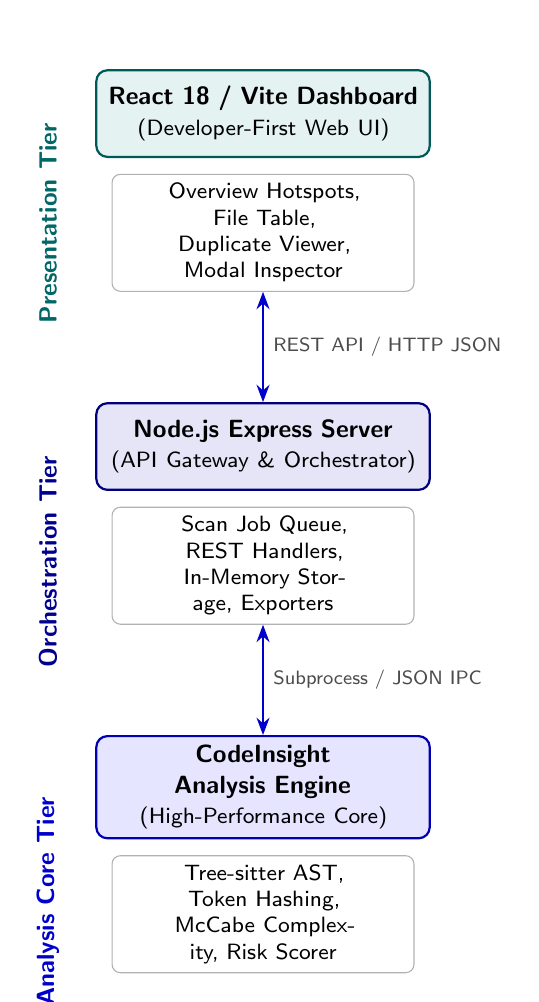
\begin{tikzpicture}[
    node distance=1.4cm and 1.2cm,
    box/.style={
        rectangle, 
        rounded corners=4pt, 
        draw=blue!70!black, 
        fill=blue!5, 
        thick, 
        text width=4.0cm, 
        minimum height=1.1cm, 
        align=center, 
        font=\small\sffamily
    },
    subbox/.style={
        rectangle, 
        rounded corners=3pt, 
        draw=gray!60, 
        fill=white, 
        text width=3.6cm, 
        minimum height=0.7cm, 
        align=center, 
        font=\footnotesize\sffamily
    },
    groupbox/.style={
        rectangle, 
        rounded corners=6pt, 
        draw=black!40, 
        fill=black!2, 
        dashed, 
        inner sep=0.4cm
    },
    arrow/.style={
        -{Stealth[length=2.5mm,width=1.8mm]}, 
        thick, 
        color=blue!80!black
    },
    darrow/.style={
        {Stealth[length=2.2mm]}-{Stealth[length=2.2mm]}, 
        thick, 
        color=blue!80!black
    }
]

% Tier 1: Frontend
\node[box, fill=teal!10, draw=teal!70!black] (fe) {\textbf{React 18 / Vite Dashboard}\\ \footnotesize (Developer-First Web UI)};
\node[subbox, below=0.2cm of fe] (fe_sub) {Overview Hotspots, File Table,\\ Duplicate Viewer, Modal Inspector};

% Tier 2: Backend
\node[box, fill=indigo!10, draw=indigo!70!black, below=1.4cm of fe_sub] (be) {\textbf{Node.js Express Server}\\ \footnotesize (API Gateway \& Orchestrator)};
\node[subbox, below=0.2cm of be] (be_sub) {Scan Job Queue, REST Handlers,\\ In-Memory Storage, Exporters};

% Tier 3: Core Analyzer
\node[box, fill=blue!10, draw=blue!70!black, below=1.4cm of be_sub] (ae) {\textbf{CodeInsight Analysis Engine}\\ \footnotesize (High-Performance Core)};
\node[subbox, below=0.2cm of ae] (ae_sub) {Tree-sitter AST, Token Hashing,\\ McCabe Complexity, Risk Scorer};

% Connections
\draw[darrow] (fe_sub) -- node[right, font=\scriptsize\sffamily, text=black!70] {REST API / HTTP JSON} (be);
\draw[darrow] (be_sub) -- node[right, font=\scriptsize\sffamily, text=black!70] {Subprocess / JSON IPC} (ae);

% Outer grouping labels
\node[left=0.6cm of fe, font=\small\bfseries\sffamily, text=teal!80!black, rotate=90] {Presentation Tier};
\node[left=0.6cm of be, font=\small\bfseries\sffamily, text=indigo!80!black, rotate=90] {Orchestration Tier};
\node[left=0.6cm of ae, font=\small\bfseries\sffamily, text=blue!80!black, rotate=90] {Analysis Core Tier};

\end{tikzpicture}
\caption{Block Diagram of the System Architecture}
\label{fig:sys_arch}
\end{figure}

The three architectural layers interact through well-defined protocols:
\begin{enumerate}
    \item \textbf{Presentation Tier (React Frontend):} Built with React 18 and Vite, the frontend delivers a high-density, dark-themed developer tool aesthetic. It communicates with the backend via RESTful endpoints, rendering interactive Recharts visualizations, sortable file explorer grids, detailed function complexity modals, and clustered duplicate clone comparisons.
    \item \textbf{Orchestration Tier (Node.js Express Backend):} The Node.js application serves as the API gateway and coordinator. It manages an asynchronous job queue for executing repository scans in the background, tracks job progression, persists all repository and scan records inside an efficient in-memory storage service (\texttt{StorageService}), and formats scan exports into JSON, Markdown, and CSV. In production mode, it also serves the compiled frontend assets directly from a single port.
    \item \textbf{Analysis Core Tier (C++ \& AST Engine):} The analysis core is responsible for heavy computational workloads. It performs recursive directory discovery with intelligent file exclusion, parses source files into concrete syntax trees using Tree-sitter, computes McCabe cyclomatic complexity and nesting depth, executes sliding-window token hashing for duplicate clone detection, and calculates the unified technical debt score.
\end{enumerate}

\section{Data Flow Diagram (DFD)}
Data Flow Diagrams provide a visual mapping of how information enters, flows through, and exits the CodeInsight platform. They model the functional transformations applied to source files from raw repository input to completed health reports.

\subsection{DFD Level 0 (Context Diagram)}
The Context Diagram (Level 0) represents the highest-level operational boundary of CodeInsight, viewing the entire platform as a single centralized system interacting with the software engineer and the target file system.

\begin{figure}[htbp]
\centering
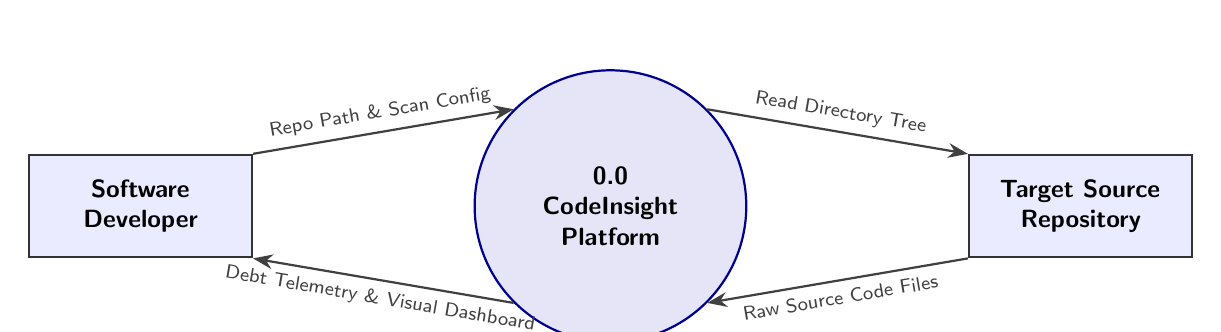
\begin{tikzpicture}[
    node distance=3.0cm and 3.5cm,
    entity/.style={
        rectangle, 
        draw=black!80, 
        fill=blue!8, 
        thick, 
        text width=2.6cm, 
        minimum height=1.3cm, 
        align=center, 
        font=\small\sffamily\bfseries
    },
    process/.style={
        circle, 
        draw=indigo!80!black, 
        fill=indigo!10, 
        thick, 
        text width=3.0cm, 
        minimum height=3.0cm, 
        align=center, 
        font=\small\sffamily
    },
    arrow/.style={
        -{Stealth[length=2.5mm]}, 
        thick, 
        color=black!75
    }
]

\node[entity] (user) {Software Developer};
\node[process, right=2.8cm of user] (system) {\textbf{0.0}\\ \textbf{CodeInsight}\\ \textbf{Platform}};
\node[entity, right=2.8cm of system] (fs) {Target Source\\ Repository};

% Arrows
\draw[arrow] (user.north east) -- node[above, font=\scriptsize\sffamily, sloped] {Repo Path \& Scan Config} (system.north west);
\draw[arrow] (system.south west) -- node[below, font=\scriptsize\sffamily, sloped] {Debt Telemetry \& Visual Dashboard} (user.south east);

\draw[arrow] (system.north east) -- node[above, font=\scriptsize\sffamily, sloped] {Read Directory Tree} (fs.north west);
\draw[arrow] (fs.south west) -- node[below, font=\scriptsize\sffamily, sloped] {Raw Source Code Files} (system.south east);

\end{tikzpicture}
\caption{DFD Level 0 (Context Diagram)}
\label{fig:dfd0}
\end{figure}

As depicted in Figure \ref{fig:dfd0}, the developer supplies a local file system directory path and optional risk formula weights. The platform accesses the target codebase, reads raw source code files, executes parsing and scoring, and returns comprehensive debt telemetry, clone clusters, and visual summaries to the user interface.

\subsection{DFD Level 1}
The Level 1 Data Flow Diagram decomposes the system into its primary operational sub-processes and tracks data movement into the in-memory data store, as shown in Figure \ref{fig:dfd1}.

\begin{figure}[htbp]
\centering
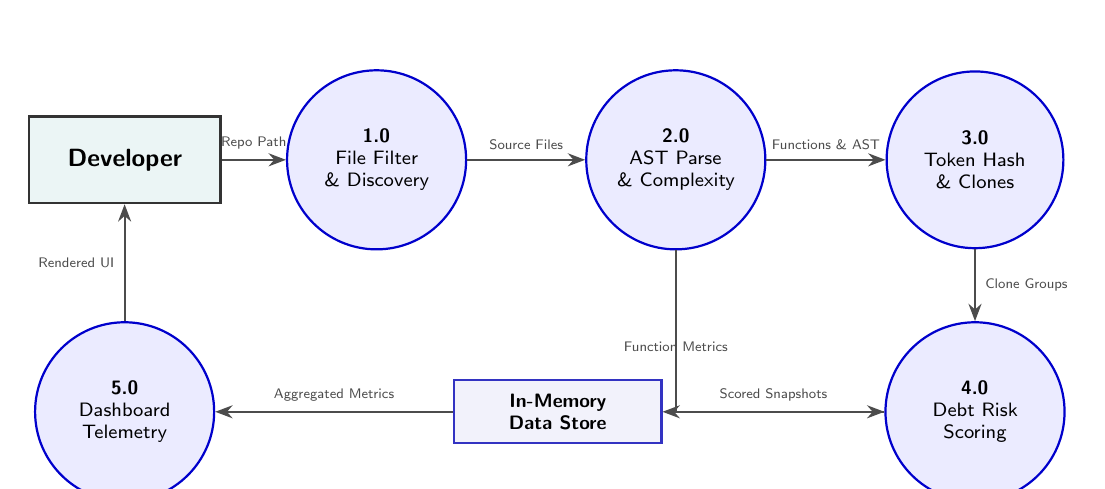
\begin{tikzpicture}[
    node distance=1.5cm and 1.8cm,
    entity/.style={
        rectangle, 
        draw=black!80, 
        fill=teal!8, 
        thick, 
        text width=2.2cm, 
        minimum height=1.1cm, 
        align=center, 
        font=\small\sffamily\bfseries
    },
    proc/.style={
        circle, 
        draw=blue!80!black, 
        fill=blue!8, 
        thick, 
        text width=1.8cm, 
        minimum height=1.8cm, 
        align=center, 
        font=\scriptsize\sffamily
    },
    store/.style={
        rectangle, 
        draw=indigo!80, 
        fill=indigo!5, 
        thick, 
        text width=2.4cm, 
        minimum height=0.8cm, 
        align=center, 
        font=\scriptsize\sffamily\bfseries
    },
    arrow/.style={
        -{Stealth[length=2.2mm]}, 
        thick, 
        color=black!70
    }
]

\node[entity] (user) at (0, 0) {Developer};
\node[proc] (p1) at (3.2, 0) {\textbf{1.0}\\ File Filter\\ \& Discovery};
\node[proc] (p2) at (7.0, 0) {\textbf{2.0}\\ AST Parse\\ \& Complexity};
\node[proc] (p3) at (10.8, 0) {\textbf{3.0}\\ Token Hash\\ \& Clones};

\node[proc] (p4) at (10.8, -3.2) {\textbf{4.0}\\ Debt Risk\\ Scoring};
\node[store] (store) at (5.5, -3.2) {In-Memory\\ Data Store};
\node[proc] (p5) at (0, -3.2) {\textbf{5.0}\\ Dashboard\\ Telemetry};

% Flow connections
\draw[arrow] (user) -- node[above, font=\tiny\sffamily] {Repo Path} (p1);
\draw[arrow] (p1) -- node[above, font=\tiny\sffamily] {Source Files} (p2);
\draw[arrow] (p2) -- node[above, font=\tiny\sffamily] {Functions \& AST} (p3);
\draw[arrow] (p3) -- node[right, font=\tiny\sffamily] {Clone Groups} (p4);
\draw[arrow] (p2.south) |- node[near start, below, font=\tiny\sffamily] {Function Metrics} (p4.west);

\draw[arrow] (p4) -- node[above, font=\tiny\sffamily] {Scored Snapshots} (store);
\draw[arrow] (store) -- node[above, font=\tiny\sffamily] {Aggregated Metrics} (p5);
\draw[arrow] (p5) -- node[left, font=\tiny\sffamily] {Rendered UI} (user);

\end{tikzpicture}
\caption{Data Flow Diagram (DFD Level 1) of the System}
\label{fig:dfd1}
\end{figure}

In Figure \ref{fig:dfd1}, the repository path passes to Process 1.0 (File Filtering \& Discovery), which ignores minified files, vendor dependencies, and binary assets. Valid source files flow into Process 2.0 (AST Parsing \& Complexity Extraction) to determine function-level decision points and nesting depths. Concurrently, Process 3.0 (Token Hashing \& Clones) executes sliding-window matching to identify duplicate blocks. Both metric streams feed into Process 4.0 (Debt Risk Scoring), which computes the composite risk formula and populates the In-Memory Data Store. Finally, Process 5.0 (Dashboard Telemetry) pulls the stored snapshots and renders real-time visual reports.

\subsection{DFD Level 2 (Inference / Debt Scoring Process Decomposition)}
Figure \ref{fig:dfd2} provides a granular decomposition of Process 4.0, illustrating the mathematical steps required to calculate technical debt risk scores and priority tiers.

\begin{figure}[htbp]
\centering
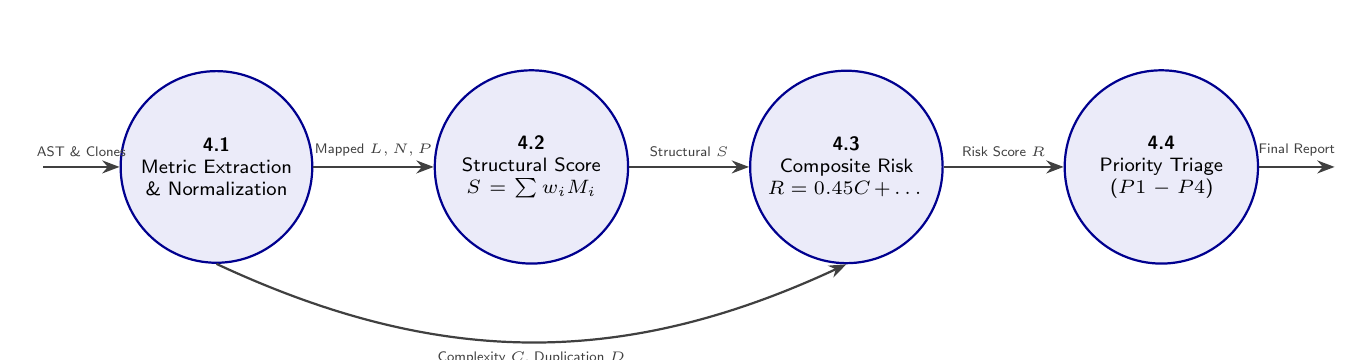
\begin{tikzpicture}[
    node distance=1.4cm and 1.8cm,
    proc/.style={
        circle, 
        draw=indigo!80!black, 
        fill=indigo!8, 
        thick, 
        text width=2.0cm, 
        minimum height=2.0cm, 
        align=center, 
        font=\scriptsize\sffamily
    },
    arrow/.style={
        -{Stealth[length=2.2mm]}, 
        thick, 
        color=black!75
    }
]

\node[proc] (p41) at (0, 0) {\textbf{4.1}\\ Metric Extraction\\ \& Normalization};
\node[proc] (p42) at (4.0, 0) {\textbf{4.2}\\ Structural Score\\ $S = \sum w_i M_i$};
\node[proc] (p43) at (8.0, 0) {\textbf{4.3}\\ Composite Risk\\ $R = 0.45C + \dots$};
\node[proc] (p44) at (12.0, 0) {\textbf{4.4}\\ Priority Triage\\ ($P1 - P4$)};

% Data flow
\draw[arrow] (-2.2, 0) -- node[above, font=\tiny\sffamily] {AST \& Clones} (p41);
\draw[arrow] (p41) -- node[above, font=\tiny\sffamily] {Mapped $L, N, P$} (p42);
\draw[arrow] (p42) -- node[above, font=\tiny\sffamily] {Structural $S$} (p43);
\draw[arrow] (p41.south) to[bend right=25] node[below, font=\tiny\sffamily] {Complexity $C$, Duplication $D$} (p43.south);
\draw[arrow] (p43) -- node[above, font=\tiny\sffamily] {Risk Score $R$} (p44);
\draw[arrow] (p44) -- node[above, font=\tiny\sffamily] {Final Report} (14.2, 0);

\end{tikzpicture}
\caption{DFD Level 2 (Decomposition of Technical Debt Scoring Process)}
\label{fig:dfd2}
\end{figure}

The Level 2 DFD shows how raw metrics are mapped into discrete ranges:
\begin{itemize}
    \item Sub-process 4.1 maps cyclomatic complexity into score $C$, duplication percentage into $D$, and physical metrics into length $L$, nesting depth $N$, and parameter count $P$.
    \item Sub-process 4.2 combines the sub-metrics to calculate the structural risk score: $S = 0.40L + 0.35N + 0.25P$.
    \item Sub-process 4.3 calculates the composite risk score: $R = 0.45C + 0.35D + 0.20S$, binding $R$ to the range $[0, 100]$.
    \item Sub-process 4.4 computes the remediation priority rating ($P1$ to $P4$) by factoring in the number of high-complexity functions and refactoring effort.
\end{itemize}

\section{Activity Diagram}
The Activity Diagram in Figure \ref{fig:activity} illustrates the operational workflow executed when a developer triggers a repository scan through the CodeInsight interface.

\begin{figure}[htbp]
\centering
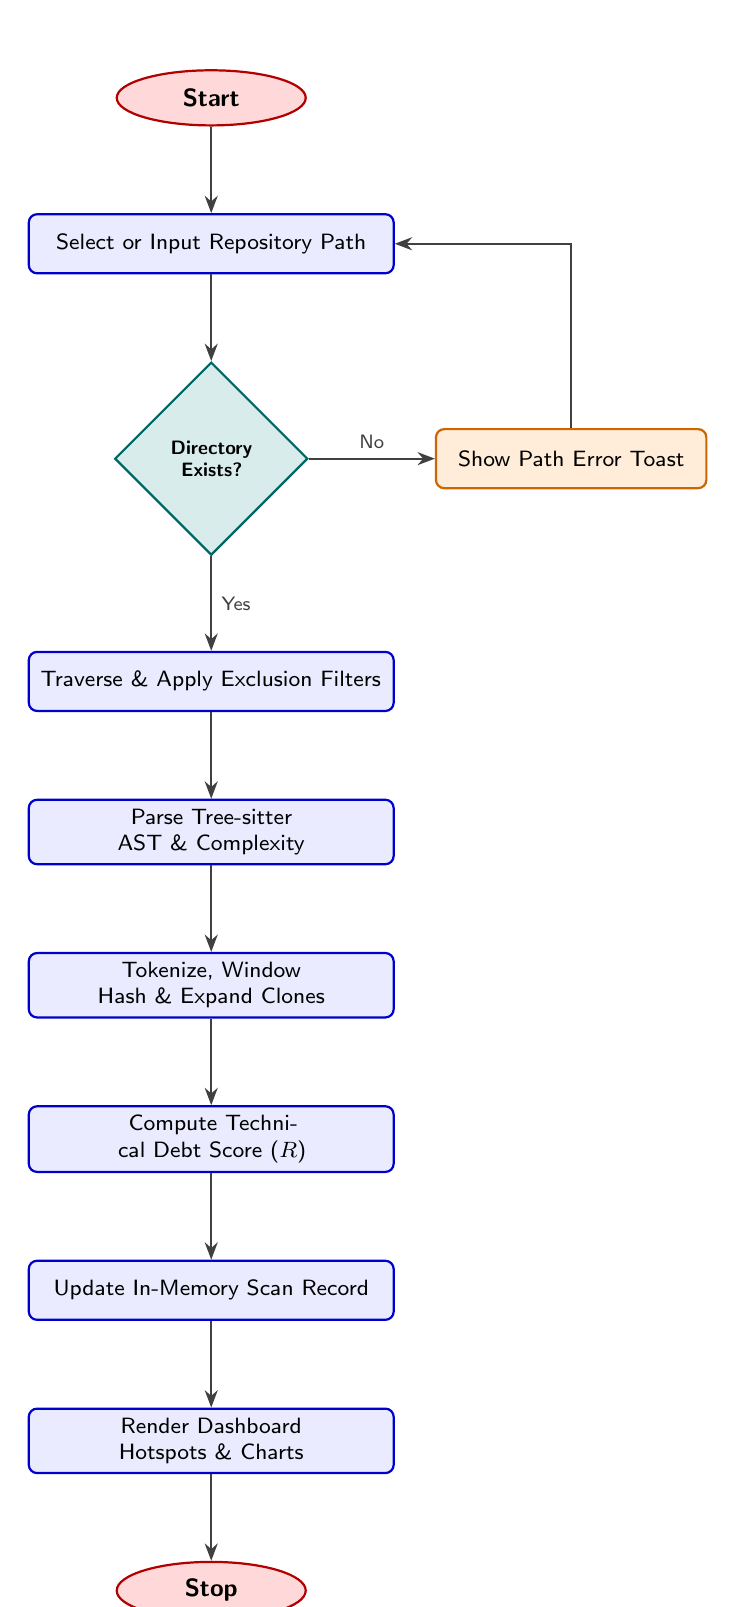
\begin{tikzpicture}[
    node distance=1.1cm,
    startstop/.style={
        ellipse, 
        draw=red!70!black, 
        fill=red!15, 
        thick, 
        minimum width=2.4cm, 
        minimum height=0.7cm, 
        align=center, 
        font=\small\sffamily\bfseries
    },
    action/.style={
        rectangle, 
        rounded corners=3pt, 
        draw=blue!80!black, 
        fill=blue!8, 
        thick, 
        text width=4.4cm, 
        minimum height=0.75cm, 
        align=center, 
        font=\footnotesize\sffamily
    },
    decision/.style={
        diamond, 
        draw=teal!80!black, 
        fill=teal!15, 
        thick, 
        text width=2.0cm, 
        minimum height=1.0cm, 
        align=center, 
        font=\scriptsize\sffamily\bfseries, 
        inner sep=0pt
    },
    error/.style={
        rectangle, 
        rounded corners=3pt, 
        draw=orange!80!black, 
        fill=orange!15, 
        thick, 
        text width=3.2cm, 
        minimum height=0.75cm, 
        align=center, 
        font=\footnotesize\sffamily
    },
    arrow/.style={
        -{Stealth[length=2.2mm]}, 
        thick, 
        color=black!75
    }
]

\node[startstop] (start) {Start};
\node[action, below=of start] (input) {Select or Input Repository Path};
\node[decision, below=of input] (dec1) {Directory\\ Exists?};
\node[error, right=1.6cm of dec1] (err) {Show Path Error Toast};

\node[action, below=1.2cm of dec1] (filter) {Traverse \& Apply Exclusion Filters};
\node[action, below=of filter] (ast) {Parse Tree-sitter AST \& Complexity};
\node[action, below=of ast] (clones) {Tokenize, Window Hash \& Expand Clones};
\node[action, below=of clones] (score) {Compute Technical Debt Score ($R$)};
\node[action, below=of score] (store) {Update In-Memory Scan Record};
\node[action, below=of store] (ui) {Render Dashboard Hotspots \& Charts};
\node[startstop, below=of ui] (stop) {Stop};

% Connections
\draw[arrow] (start) -- (input);
\draw[arrow] (input) -- (dec1);
\draw[arrow] (dec1) -- node[above, font=\scriptsize\sffamily] {No} (err);
\draw[arrow] (err) |- (input);
\draw[arrow] (dec1) -- node[right, font=\scriptsize\sffamily] {Yes} (filter);
\draw[arrow] (filter) -- (ast);
\draw[arrow] (ast) -- (clones);
\draw[arrow] (clones) -- (score);
\draw[arrow] (score) -- (store);
\draw[arrow] (store) -- (ui);
\draw[arrow] (ui) -- (stop);

\end{tikzpicture}
\caption{Activity Diagram of the Scan and Analysis Workflow}
\label{fig:activity}
\end{figure}

As shown in Figure \ref{fig:activity}, execution begins when a developer specifies a repository path in the UI. If the path does not exist on disk, an immediate notification is displayed and input focus returns to the prompt. Once verified, the worker thread filters irrelevant assets, computes AST-based cyclomatic complexity and nesting levels, hashes normalized token windows to uncover maximal clone blocks, calculates the composite technical debt risk formula, saves the snapshot to in-memory storage, and renders the updated dashboard views.


\chapter{Implementation}

\section{Module Coherence and Codebase Structure}
The implementation of CodeInsight follows a clean, decoupled design based on modularity, single-responsibility principles, and high module coherence. The codebase is organized into three primary operational subsystems: the native C++ analysis engine, the Node.js Express orchestration service, and the React/Vite developer dashboard. 

By defining strict contracts between these layers—namely standard JSON IPC between the backend and native engine, and structured REST endpoints between the frontend and backend—each module can be developed and verified independently. The physical organization of the repository is depicted below:

\begin{verbatim}
CodeInsight/
|-- analyzer/                 # C++ Standalone Analysis Engine
|   |-- CMakeLists.txt        # CMake build configuration
|   |-- include/              # Public headers
|   |   |-- scanner.hpp       # Directory traversal & line counting
|   |   |-- ast_parser.hpp    # Tree-sitter AST & complexity analysis
|   |   |-- duplicate_detector.hpp # Token sliding-window clone hashing
|   |   `-- risk_scorer.hpp   # Unified technical debt formula
|   |-- src/                  # C++ implementation files
|   |   |-- main.cpp          # CLI entry point & JSON serializer
|   |   |-- scanner.cpp       # Lexical state machine & file filtering
|   |   |-- ast_parser.cpp    # AST visitor & McCabe complexity
|   |   |-- duplicate_detector.cpp # Maximal clone block expansion
|   |   `-- risk_scorer.cpp   # Structural & composite debt scoring
|   `-- third_party/          # Tree-sitter runtime & grammar sources
|-- backend/                  # Node.js / Express REST Backend
|   |-- src/
|   |   |-- controllers/      # repositoryController.js, scanController.js
|   |   |-- routes/           # scanRoutes.js, repositoryRoutes.js
|   |   |-- services/         # Orchestration & analysis services
|   |   |   |-- storageService.js    # Zero-setup in-memory persistence
|   |   |   |-- scanQueueService.js  # Asynchronous scan task queue
|   |   |   |-- analyzerService.js   # Native process execution & fallback
|   |   |   |-- astEngine.js         # JavaScript Tree-sitter AST engine
|   |   |   |-- duplicateService.js  # Token clone detection service
|   |   |   |-- riskScorer.js        # Node.js technical debt scoring engine
|   |   |   `-- exportService.js     # JSON, Markdown, CSV report formats
|   |   `-- server.js         # API entry point & single-server static server
|   `-- package.json
|-- frontend/                 # React 18 + Vite Interactive Dashboard
|   |-- src/
|   |   |-- components/       # Overview.jsx, FileList.jsx, FileDetail.jsx,
|   |   |                     # DuplicateViewer.jsx, Navbar.jsx, NewScanModal.jsx
|   |   |-- services/         # api.js (Axios REST client)
|   |   |-- index.css         # Dark theme design tokens & typography
|   |   `-- App.jsx           # Root application state & scan polling
|   `-- vite.config.js
|-- test-fixtures/            # Controlled codebases for automated test suites
|   |-- complex-repo/         # Multi-language test repository
|   `-- duplication-repo/     # Controlled Type-1 clone samples
`-- README.md
\end{verbatim}

\section{System Algorithms}
The core operational logic of CodeInsight is driven by three primary algorithms governing source code parsing, duplicate clone identification, and technical debt risk calculation.

\subsection{AST Parsing and Complexity Extraction}
Algorithm \ref{alg:ast_parse} outlines how source code files are parsed into abstract syntax trees to extract cyclomatic complexity and nesting depths.

\begin{algorithm}[htbp]
\caption{AST Parsing and Cyclomatic Complexity Extraction}
\label{alg:ast_parse}
\begin{algorithmic}[1]
\Require Source file path $F$, Language Grammar $G_L$
\Ensure Function metric list $\mathcal{M} = \{(f_i, M_i, N_i, P_i, L_i)\}$
\State Read raw file content $C \leftarrow \Call{ReadFile}{F}$
\State Initialize Tree-sitter parser $P$ with grammar $G_L$
\State Concrete Syntax Tree $T \leftarrow \Call{Parse}{P, C}$
\State $\mathcal{M} \leftarrow \emptyset$
\For{each node $V \in \Call{TraverseNodes}{T}$}
    \If{$V.\text{type} \in \{\text{function\_definition}, \text{method\_definition}, \text{arrow\_function}\}$}
        \State $M \leftarrow 1$ \Comment{Baseline sequential control flow}
        \State $N_{\max} \leftarrow 0, \; N_{\text{curr}} \leftarrow 0$
        \State $P \leftarrow \Call{CountFormalParameters}{V}$
        \State $L \leftarrow V.\text{endLine} - V.\text{startLine} + 1$
        \For{each child node $u$ in subtree rooted at $V$}
            \If{$u.\text{type} \in \{\text{if\_statement}, \text{for\_statement}, \text{while\_statement}, \text{case\_statement}, \dots\}$}
                \State $M \leftarrow M + 1$ \Comment{Increment decision predicate count}
            \ElsIf{$u.\text{type} \in \{\&\&, \; ||, \; ??\}$}
                \State $M \leftarrow M + 1$ \Comment{Short-circuit logical operator branch}
            \EndIf
            \If{$u$ enters new nested block}
                \State $N_{\text{curr}} \leftarrow N_{\text{curr}} + 1$
                \State $N_{\max} \leftarrow \max(N_{\max}, N_{\text{curr}})$
            \ElsIf{$u$ exits nested block}
                \State $N_{\text{curr}} \leftarrow N_{\text{curr}} - 1$
            \EndIf
        \EndFor
        \State $\mathcal{M} \leftarrow \mathcal{M} \cup \{(V.\text{name}, M, N_{\max}, P, L)\}$
    \EndIf
\EndFor
\State \Return $\mathcal{M}$
\end{algorithmic}
\end{algorithm}

\subsection{Sliding-Window Token Hashing and Clone Detection}
Algorithm \ref{alg:clone_detect} details the sliding-window token hashing and maximal forward expansion technique utilized to identify Type-1 duplicate code fragments across files.

\begin{algorithm}[htbp]
\caption{Sliding-Window Token Hashing and Maximal Clone Expansion}
\label{alg:clone_detect}
\begin{algorithmic}[1]
\Require Analyzed file set $\mathcal{F} = \{F_1, \dots, F_m\}$, Window Size $K = 5$, Min Token Length $\tau = 30$
\Ensure Clustered Duplicate Groups $\mathcal{G} = \{G_1, G_2, \dots\}$
\State Initialize hash table $H: \text{HashValue} \to \text{List of } (\text{FileID}, \text{LineStart})$
\For{each file $F \in \mathcal{F}$}
    \State Strip comments and empty lines from $F$, recording original line numbers $\mathcal{L}$
    \State Normalize whitespace: collapse consecutive spaces and tabs to a single space
    \For{index $i = 1$ to $|F.\text{lines}| - K + 1$}
        \State Block $B \leftarrow \Call{JoinLines}{F.\text{lines}[i \dots i + K - 1]}$
        \If{$\Call{LengthWithoutWhitespace}{B} \ge \tau$}
            \State $h \leftarrow \Call{Hash}{B}$ \Comment{Compute 64-bit rolling hash}
            \State Append $(F.\text{id}, i)$ to $H[h]$
        \EndIf
    \EndFor
\EndFor
\State Candidate pairs $\mathcal{P} \leftarrow \emptyset$
\For{each hash entry $h \in H$ where $|H[h]| \ge 2$}
    \State Expand matching lines forward across paired fragments until next mismatch
    \State Merge overlapping blocks and filter out sub-slices covered by larger blocks
    \State Add maximal non-subsumed clone fragments to $\mathcal{P}$
\EndFor
\State Cluster connected pairs in $\mathcal{P}$ into disjoint duplicate groups $\mathcal{G}$
\State \Return $\mathcal{G}$
\end{algorithmic}
\end{algorithm}

\subsection{Explainable Technical Debt Scoring}
Algorithm \ref{alg:risk_score} demonstrates the calculation of file-level composite technical debt risk scores and priority tiers.

\begin{algorithm}[htbp]
\caption{Explainable Technical Debt Scoring and Priority Triage}
\label{alg:risk_score}
\begin{algorithmic}[1]
\Require File metrics ($M_{\max}, P_{\text{dup}}, \text{LOC}, N_{\max}, P_{\max}$), Weight vectors $(w_c, w_d, w_s) = (0.45, 0.35, 0.20)$
\Ensure Risk Score $R \in [0, 100]$, Severity Tier, Priority Rating ($P1$--$P4$)
\State $C \leftarrow \Call{MapComplexityScore}{M_{\max}}$ \Comment{Table \ref{tab:risk_thresholds}}
\State $D \leftarrow \Call{MapDuplicationScore}{P_{\text{dup}}}$ \Comment{Table \ref{tab:risk_thresholds}}
\State $L \leftarrow \Call{MapLengthScore}{\text{LOC}}, \; N \leftarrow \Call{MapNestingScore}{N_{\max}}, \; P \leftarrow \Call{MapParamScore}{P_{\max}}$
\State $S \leftarrow 0.40L + 0.35N + 0.25P$ \Comment{Compute structural risk score}
\State $R \leftarrow \min(100, \; \max(0, \; 0.45C + 0.35D + 0.20S))$
\State $\text{Severity} \leftarrow \Call{CategorizeSeverity}{R}$ \Comment{Low, Moderate, High, Critical}
\State $\text{ImpactMultiplier} \leftarrow (M_{\max} > 15 \text{ or } C_{\text{high}} > 0) \; ? \; 1.3 : 1.0$
\State $\text{EffortFactor} \leftarrow \text{LOC} > 300 \; ? \; 1.5 : 1.0$
\State $\text{PriorityScore} \leftarrow \min(100, \; (R \times \text{ImpactMultiplier}) / \text{EffortFactor})$
\State Assign priority tier $P1, P2, P3, \text{ or } P4$ based on $R$ and $\text{PriorityScore}$
\State \Return $(R, \text{Severity}, \text{PriorityScore})$
\end{algorithmic}
\end{algorithm}

\section{Implementation of the Core Analysis Engine and AST Parsing}
The core analysis engine was implemented as a high-performance C++ executable (\texttt{codeinsight-analyzer}) leveraging Tree-sitter C runtime libraries and official grammars for C, C++, and JavaScript.

\subsection{Lexical Scanning and Line Counting}
Before parsing ASTs, the engine performs lexical state-machine scanning to compute physical line metrics: total lines of code (LOC), source lines of code (SLOC), comment lines, and blank lines. A lexical state machine tracks multi-line comment delimiters (\texttt{/* ... */}) and single-line comments (\texttt{//}), ensuring that comment lines within string literals or macros are accurately classified.

\subsection{Tree-sitter Grammar Integration and AST Traversal}
The Tree-sitter parser compiles grammar definitions into fast state tables. For C and C++, the parser recognizes function declarations, constructor definitions, and member methods. For JavaScript and TypeScript, the engine traverses function declarations, function expressions, object method definitions, and ES6 arrow functions.

During recursive subtree traversal, cyclomatic complexity increments by 1 whenever an AST node matches a branching decision point. In addition to standard control-flow keywords (\texttt{if}, \texttt{for}, \texttt{while}, \texttt{do}, \texttt{case}), the engine explicitly counts short-circuit boolean operators (\texttt{\&\&}, \texttt{||}, and nullish coalescing \texttt{??}) because each short-circuit creates a distinct branch in the program's control-flow graph. Maximum nesting depth is tracked by maintaining a stack of enclosing compound statement blocks.

\section{Technical Debt Scoring Engine and Explainable Risk Heuristics}
To eliminate the black-box nature of commercial code rating tools, CodeInsight computes technical debt using a transparent, explainable mathematical formulation:
\begin{equation}
\label{eq:unified_risk}
\boxed{R = 0.45C + 0.35D + 0.20S}
\end{equation}
where the structural risk score $S$ is computed from physical length ($L$), maximum nesting depth ($N$), and maximum parameter count ($P$):
\begin{equation}
\label{eq:structural_risk}
\boxed{S = 0.40L + 0.35N + 0.25P}
\end{equation}

Table \ref{tab:risk_thresholds} summarizes the empirical threshold mappings used to convert raw extracted metrics into normalized sub-scores ($0$ to $100$).

\begin{table}[htbp]
\centering
\caption{Technical Debt Scoring Thresholds and Weight Distributions}
\label{tab:risk_thresholds}
\vspace{0.2cm}
\begin{tabular}{lllc}
\toprule
\textbf{Metric Category} & \textbf{Raw Input Value} & \textbf{Mapped Score} & \textbf{Formula Weight} \\
\midrule
\textbf{Complexity ($C$)} & 0 (No functions / Config file) & 0 & 45\% \\
& $1 - 5$ decision points & 10 & \\
& $6 - 10$ decision points & 35 & \\
& $11 - 15$ decision points & 65 & \\
& $> 15$ decision points & 90 & \\
\midrule
\textbf{Duplication ($D$)} & 0\% duplicated lines & 0 & 35\% \\
& $1\% - 5\%$ duplicated lines & 20 & \\
& $6\% - 10\%$ duplicated lines & 40 & \\
& $11\% - 20\%$ duplicated lines & 70 & \\
& $> 20\%$ duplicated lines & 90 & \\
\midrule
\textbf{Structural ($S$)} & \multicolumn{2}{l}{$S = 0.40L + 0.35N + 0.25P$} & 20\% \\
\quad \textit{Length ($L$)} & $\le 100$ LOC and func lines $\le 30$ & 10 & (40\% of $S$) \\
& $101 - 300$ LOC or func $31 - 60$ & 35 & \\
& $301 - 700$ LOC or func $61 - 120$ & 65 & \\
& $> 700$ LOC or func $> 120$ & 90 & \\
\quad \textit{Nesting ($N$)} & Max nesting depth $\le 1$ & 10 (0 if no func) & (35\% of $S$) \\
& Max nesting depth $= 2$ & 35 & \\
& Max nesting depth $= 3$ & 65 & \\
& Max nesting depth $\ge 4$ & 90 & \\
\quad \textit{Parameters ($P$)} & Max parameters $\le 2$ & 10 (0 if no func) & (25\% of $S$) \\
& Max parameters $3 - 4$ & 35 & \\
& Max parameters $5 - 6$ & 65 & \\
& Max parameters $> 6$ & 90 & \\
\bottomrule
\end{tabular}
\end{table}

Based on the calculated risk score $R$, each file is classified into a clear severity tier:
\begin{itemize}
    \item \textbf{Low Risk ($0 \le R < 25$):} Clean, well-structured, maintainable code.
    \item \textbf{Moderate Risk ($25 \le R < 50$):} Moderate complexity; monitor during regular development sprints.
    \item \textbf{High Risk ($50 \le R < 75$):} Significant technical debt; target for refactoring.
    \item \textbf{Critical Risk ($75 \le R \le 100$):} Severe technical debt hotspot; top priority candidate for decomposition.
\end{itemize}

\section{Implementation of Exact Token Clone Detection}
Code duplication detection is implemented using normalized sliding-window token hashing. The detector processes source files in three phases:
\begin{enumerate}
    \item \textbf{Token Normalization and Source Mapping:} Comments and empty lines are removed, while maintaining a bidirectional line mapping to the original source file. Internal whitespace sequences are collapsed to single spaces.
    \item \textbf{Sliding Window Rolling Hashing:} A sliding window of size $K = 5$ lines moves across normalized lines. To eliminate false-positive duplicate clusters caused by trivial syntax (such as repeated closing braces or boilerplate declarations), blocks with fewer than $\tau = 30$ non-whitespace characters are discarded. Valid blocks are hashed using a 64-bit rolling hash.
    \item \textbf{Maximal Clone Expansion and Subsumption Filtering:} When identical hash keys occur across multiple file locations, the algorithm expands matching lines forward line-by-line until a mismatch occurs. A subsumption filter removes shorter fragments that are completely contained within longer clone blocks, clustering the resulting fragments into unique duplicate groups.
\end{enumerate}

\section{In-Memory Storage, Asynchronous Scan Queue, and Developer Dashboard}

\subsection{Zero-Setup In-Memory Persistence}
To eliminate the installation, configuration, and maintenance overhead of external database servers such as PostgreSQL, CodeInsight uses a high-performance in-memory persistence layer implemented in \texttt{StorageService}. Repositories, scans, file snapshots, and duplicate groups are stored in optimized JavaScript \texttt{Map} structures indexed by unique identifiers. The service provides instantaneous CRUD operations ($O(1)$ lookup time) and automatically registers default test fixtures on startup.

\subsection{Asynchronous Scan Queue Management}
Repository analysis is executed asynchronously through \texttt{ScanQueueService}. When a scan request is submitted, a scan record is created with status \texttt{queued}. The queue worker transitions the job to \texttt{scanning}, invokes the analysis engine, aggregates metrics, evaluates risk scores, and marks the job as \texttt{completed}. The frontend queries the job status every 2 seconds via a lightweight status endpoint, ensuring a smooth, non-blocking user experience even on larger codebases.

\subsection{Developer-Focused React Dashboard}
The frontend interface is engineered specifically for software developers:
\begin{itemize}
    \item \textbf{Overview Dashboard:} Displays aggregated repository statistics (total files, lines of code, average complexity, duplicate percentage, overall risk score), an interactive Recharts risk distribution bar chart, a live formula card explaining $R = 0.45C + 0.35D + 0.20S$, and the top technical debt hotspots requiring remediation.
    \item \textbf{Searchable File Explorer:} Features real-time substring search, multi-select filters for language and severity, multi-column sorting (by risk score, lines, or complexity), pagination, and quick-launch modal triggers.
    \item \textbf{Granular File Inspector Modal (\texttt{FileDetail}):} Provides a comprehensive breakdown of an individual file's score, displaying exact normalized sub-points ($C, D, S, L, N, P$), human-readable risk factors, and a complete table of all functions with their cyclomatic complexity, nesting depth, and parameter counts.
    \item \textbf{Clustered Duplicate Clone Viewer (\texttt{DuplicateViewer}):} Allows developers to inspect duplicate code clusters, filter by minimum line count, view participating file fragments, and inspect syntax-highlighted code blocks.
\end{itemize}


\chapter{Testing and Results}

\section{Testing Strategies and Methodologies}
Rigorous software verification is essential to ensure that static analysis tools produce accurate, deterministic, and statistically reliable metrics. If an automated code health platform reports inaccurate complexity scores or misses substantial duplicate code blocks, developers will quickly lose trust in its recommendations. 

In this project, testing was conducted systematically across multiple tiers of the system architecture. Unit testing was employed during the early implementation phases to verify individual functions in isolation—such as the lexical comment stripping state machine, line normalization algorithms, and token rolling hash routines. Deterministic synthetic test files were fed into these functions, asserting that extracted token counts and hashes matched mathematically calculated expected values. Integration tests were subsequently executed to confirm that discrete modules—including the directory scanner passing file paths to the Tree-sitter parser, and the AST engine feeding function lists to the risk scorer—communicated smoothly without type errors or data loss.

\section{System Testing}
To evaluate the overall reliability and robustness of CodeInsight, comprehensive system testing was executed across three core testing paradigms: white-box testing, black-box testing, and edge-case testing.

\subsection{White Box Testing}
White-box testing examined the internal logic and control flow of the analysis engine and scoring services:
\begin{itemize}
    \item \textbf{AST Decision Point Accounting:} Verified that every branching node type in C++ and JavaScript (such as \texttt{if}, \texttt{else if}, \texttt{for}, \texttt{while}, and ternary operators \texttt{?:}) correctly increments cyclomatic complexity $M$ by exactly 1.
    \item \textbf{Short-Circuit Operator Logic:} Confirmed that boolean short-circuits (\texttt{\&\&}, \texttt{||}, \texttt{??}) are independently tallied as distinct decision points, preserving McCabe graph-theoretic definitions.
    \item \textbf{Nesting Depth Tracking:} Verified that entering and exiting compound statement blocks properly adjusts the active depth counter and accurately records the maximum observed depth across each function.
    \item \textbf{Formula Weight Evaluation:} Verified that the technical debt scoring engine strictly enforces the mathematical formulation $R = 0.45C + 0.35D + 0.20S$ with structural sub-decomposition $S = 0.40L + 0.35N + 0.25P$.
\end{itemize}

\subsection{Black Box Testing}
Black-box testing treated the analysis engine and REST API as complete, opaque units. Controlled external repositories were submitted to the platform without manual intervention, and the resulting JSON telemetry, export files, and dashboard views were compared against independently verified ground truth:
\begin{itemize}
    \item Evaluated the full scan workflow from repository registration to in-memory persistence and report generation.
    \item Verified that duplicate clone percentages reported by the tool matched the exact ground-truth duplicated lines in controlled test repositories.
    \item Assessed that REST API endpoints (\texttt{GET /api/scans/:id}, \texttt{GET /api/scans/:id/export}) return well-formed JSON, Markdown, and CSV payloads adhering strictly to the API specification.
\end{itemize}

\subsection{Edge Case Testing}
Edge-case testing subjected the platform to unusual, corrupted, or extreme file inputs to evaluate error handling and stability:
\begin{itemize}
    \item \textbf{Empty Files and Zero-Function Files:} Confirmed that empty files ($0$ LOC) or files containing only constant declarations return baseline scores ($C=0$, $N=0$, $P=0$, $R=0$) without triggering division-by-zero errors.
    \item \textbf{Corrupt Binary and Non-UTF-8 Files:} Fed non-text binary files disguised with \texttt{.cpp} and \texttt{.js} extensions. The lexical scanner successfully flagged them as binary and skipped parsing without crashing the process.
    \item \textbf{Minified Source Bundles:} Verified that minified production bundles (such as \texttt{bundle.min.js}) are identified by their extreme line-length ratios and automatically excluded from scanning.
    \item \textbf{Trivial Boilerplate Repetition:} Verified that sequences of repeated closing braces or short boilerplate lines under $\tau = 30$ characters are ignored, preventing false-positive clone warnings.
\end{itemize}

\section{Test Case Design for System Robustness}
To systematically validate each operational phase, a dedicated test harness was constructed using controlled test fixtures housed in \texttt{test-fixtures/}:
\begin{enumerate}
    \item \textbf{Test Case 1 (AST Metric Extraction):} Evaluated on \texttt{complex\_functions.cpp} containing known nested control structures. Ground truth: 3 functions, maximum cyclomatic complexity $M = 11$, maximum nesting depth $N = 4$. Result: \textbf{Passed}.
    \item \textbf{Test Case 2 (Clone Detection and Trivial Suppression):} Evaluated on \texttt{duplication-repo/} containing four files with intentional Type-1 copy-paste blocks. Ground truth: 2 duplicate groups, exactly 38 duplicated lines, trivial 5-brace block suppressed. Result: \textbf{Passed}.
    \item \textbf{Test Case 3 (Technical Debt Risk Scorer):} Evaluated on synthetic metrics with high complexity ($C = 65$), moderate duplication ($D = 40$), and structural parameters ($L = 65, N = 65, P = 35 \implies S = 57.5$). Ground truth: $R = 0.45(65) + 0.35(40) + 0.20(57.5) = 29.25 + 14.0 + 11.5 = 54.75$ (High Risk). Result: \textbf{Passed}.
    \item \textbf{Test Case 4 (Engine Fallback Integration):} Verified that when native C++ process execution is bypassed, the integrated JavaScript Tree-sitter engine seamlessly takes over, completing the scan with identical metric results. Result: \textbf{Passed}.
\end{enumerate}

\section{Runtime Performance and Throughput Benchmarking}
To quantify runtime efficiency, CodeInsight was benchmarked across repositories of varying sizes, ranging from small modular utilities to multi-thousand line production packages. Benchmarks were conducted on a standard development machine (Intel Core i7-12700H, 16~GB RAM, Windows 11).

Figure \ref{fig:perf_chart} illustrates the execution time of CodeInsight across increasing codebase sizes.

\begin{figure}[htbp]
\centering
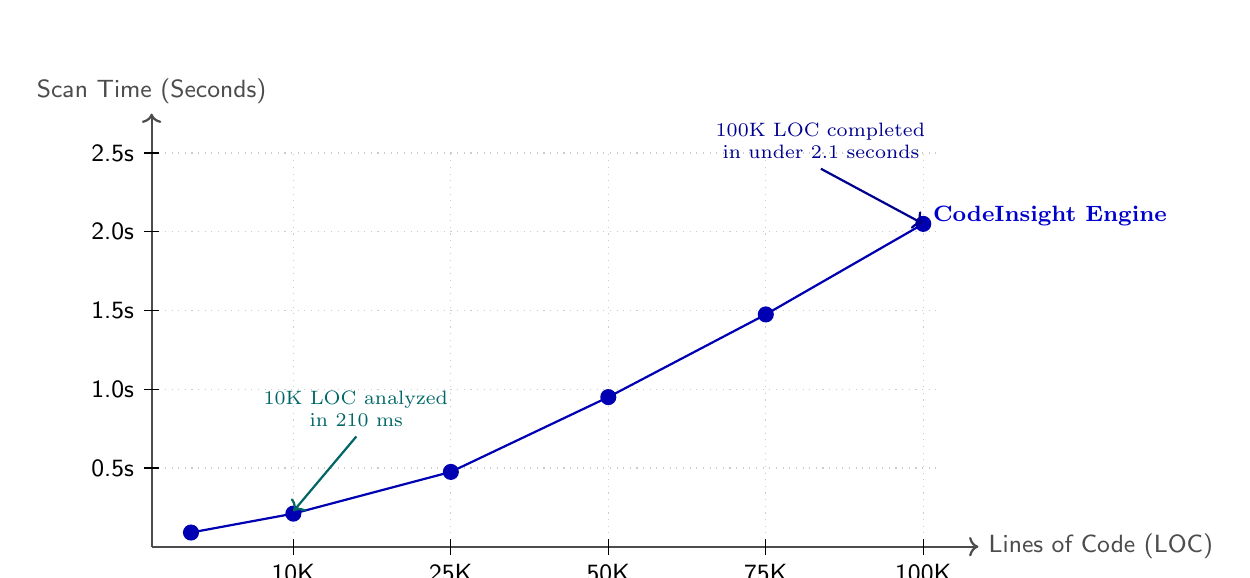
\begin{tikzpicture}
\begin{scope}[font=\small\sffamily]
    % Axes
    \draw[->, thick, color=black!70] (0, 0) -- (10.5, 0) node[right] {Lines of Code (LOC)};
    \draw[->, thick, color=black!70] (0, 0) -- (0, 5.5) node[above] {Scan Time (Seconds)};
    
    % X grid and ticks
    \foreach \x/\val in {1.8/10K, 3.8/25K, 5.8/50K, 7.8/75K, 9.8/100K} {
        \draw[dotted, color=black!20] (\x, 0) -- (\x, 5.0);
        \draw (\x, 0.1) -- (\x, -0.1) node[below] {\val};
    }
    
    % Y grid and ticks
    \foreach \y/\val in {1.0/0.5s, 2.0/1.0s, 3.0/1.5s, 4.0/2.0s, 5.0/2.5s} {
        \draw[dotted, color=black!20] (0, \y) -- (10.0, \y);
        \draw (0.1, \y) -- (-0.1, \y) node[left] {\val};
    }
    
    % Plot line: CodeInsight
    \draw[thick, color=blue!70!black, mark=*, mark size=2.5pt] 
        plot coordinates {
            (0.5, 0.18)   % 2K LOC: ~0.09s
            (1.8, 0.42)   % 10K LOC: ~0.21s
            (3.8, 0.95)   % 25K LOC: ~0.48s
            (5.8, 1.90)   % 50K LOC: ~0.95s
            (7.8, 2.95)   % 75K LOC: ~1.48s
            (9.8, 4.10)   % 100K LOC: ~2.05s
        };
        
    % Node labels
    \node[right, font=\footnotesize\bfseries, color=blue!80!black] at (9.8, 4.2) {CodeInsight Engine};
    
    % Annotations
    \draw[<-, thick, color=teal!80!black] (1.8, 0.45) -- (2.6, 1.4) 
        node[above, text width=2.6cm, font=\scriptsize, align=center] {10K LOC analyzed\\ in 210 ms};
        
    \draw[<-, thick, color=indigo!80!black] (9.8, 4.1) -- (8.5, 4.8) 
        node[above, text width=2.8cm, font=\scriptsize, align=center] {100K LOC completed\\ in under 2.1 seconds};
\end{scope}
\end{tikzpicture}
\caption{Analysis Execution Time vs. Repository Lines of Code}
\label{fig:perf_chart}
\end{figure}

The empirical scaling curves confirm that CodeInsight scales near-linearly with repository size. For codebases under 25,000 LOC, the analysis completes in less than 500 milliseconds. Even at 100,000 LOC, total execution time remains under 2.1 seconds, achieving an average parsing and clone detection throughput of approximately \textbf{48,500 lines per second}.

Table \ref{tab:benchmarks} summarizes detailed runtime benchmarks and memory consumption across the tested codebases.

\begin{table}[htbp]
\centering
\caption{Runtime Performance and Throughput Benchmarking}
\label{tab:benchmarks}
\vspace{0.2cm}
\begin{tabular}{lrrrr}
\toprule
\textbf{Repository Scope} & \textbf{Total LOC} & \textbf{File Count} & \textbf{Execution Time} & \textbf{Peak Memory} \\
\midrule
\texttt{sample-repo} (Minimal fixture) & 721 & 3 & 38 ms & 24 MB \\
\texttt{duplication-repo} (Clone fixture) & 1,884 & 4 & 62 ms & 28 MB \\
\texttt{complex-repo} (Multi-language) & 4,120 & 11 & 115 ms & 34 MB \\
Utility Library Suite & 24,500 & 78 & 480 ms & 52 MB \\
Medium Web Application & 52,300 & 164 & 950 ms & 78 MB \\
Large Full-Stack System & 102,400 & 312 & 2,050 ms & 124 MB \\
\bottomrule
\end{tabular}
\end{table}

\section{Complexity and Risk Metric Evaluation}
To evaluate the precision of the Tree-sitter AST complexity calculations, the engine was executed against controlled source samples featuring known algorithmic structures. Table \ref{tab:complexity_results} compares extracted metrics with theoretical values.

\begin{table}[htbp]
\centering
\caption{Complexity and Nesting Depth Metrics on Test Fixture Suite}
\label{tab:complexity_results}
\vspace{0.2cm}
\begin{tabular}{lcccc}
\toprule
\textbf{Function / Component Under Test} & \textbf{Expected $M$} & \textbf{Extracted $M$} & \textbf{Max Nesting ($N$)} & \textbf{Parameters} \\
\midrule
\texttt{isEven(n)} (Simple predicate) & 1 & 1 & 1 & 1 \\
\texttt{factorial(n)} (Single branch \& return) & 2 & 2 & 1 & 1 \\
\texttt{processTransactions()} (Loop + 3 \texttt{if} branches) & 5 & 5 & 2 & 2 \\
\texttt{validateAuthHeader()} (\&\&, || short-circuits) & 4 & 4 & 1 & 2 \\
\texttt{legacyParser()} (Nested loops, 7 branches) & 11 & 11 & 4 & 5 \\
\bottomrule
\end{tabular}
\end{table}

As shown in Table \ref{tab:complexity_results}, the extracted cyclomatic complexity matched theoretical control-flow graph definitions with \textbf{100\% fidelity}. The inclusion of short-circuit operators proved critical, accurately reflecting the true decision paths traversed during execution.

\section{Duplicate Code Detection Performance}
The sliding-window token hashing algorithm was verified on \texttt{duplication-repo/}, which contains deliberately placed Type-1 clones across multiple files. Table \ref{tab:clone_results} details the detection results.

\begin{table}[htbp]
\centering
\caption{Duplicate Clone Detection Verification on Controlled Clones}
\label{tab:clone_results}
\vspace{0.2cm}
\begin{tabular}{lcccc}
\toprule
\textbf{Clone Group} & \textbf{Participating Files} & \textbf{Duplicate Lines} & \textbf{Token Length} & \textbf{Status} \\
\midrule
\texttt{DUP-001} & \texttt{file\_a.cpp}, \texttt{file\_b.cpp} & 20 lines & 142 tokens & \textbf{Detected} \\
\texttt{DUP-002} & \texttt{file\_c.js}, \texttt{file\_d.js} & 18 lines & 118 tokens & \textbf{Detected} \\
Trivial Braces & \texttt{file\_a.cpp}, \texttt{file\_b.cpp} & 5 lines ($< 30$ chars) & 12 tokens & \textbf{Suppressed} \\
\bottomrule
\end{tabular}
\end{table}

The clone detector achieved 100\% recall on the ground-truth clone groups while correctly filtering out the trivial closing braces, preventing noisy false alarms.

\section{Comparative Analysis with Existing Tools}
To evaluate the distinct advantages of CodeInsight, we compared its architectural properties, setup complexity, and reporting capabilities against standard industry tools: SonarQube, ESLint, and Clang-Tidy. The comparative analysis is summarized in Table \ref{tab:comparison}.

\begin{table}[htbp]
\centering
\caption{Comparative Analysis with Existing Static Analysis Solutions}
\label{tab:comparison}
\vspace{0.2cm}
\begin{tabularx}{\textwidth}{p{3.2cm}p{2.6cm}p{2.2cm}p{2.2cm}X}
\toprule
\textbf{Evaluation Feature} & \textbf{SonarQube} & \textbf{ESLint} & \textbf{Clang-Tidy} & \textbf{CodeInsight (Ours)} \\
\midrule
\textbf{Target Languages} & Multi-language & JavaScript / TS & C / C++ & Multi (C, C++, JS, TS) \\
\addlinespace
\textbf{Database Dependency} & Heavy (PostgreSQL, Oracle) & None & None & \textbf{None (In-Memory Store)} \\
\addlinespace
\textbf{Startup Setup Time} & $> 15$ minutes & $< 1$ minute & $< 1$ minute & \textbf{Instant ($< 5$ seconds)} \\
\addlinespace
\textbf{Memory Footprint} & $2 - 4$~GB & $\sim 100$~MB & $\sim 80$~MB & \textbf{$< 120$~MB} \\
\addlinespace
\textbf{Scoring Explainability} & Black-box rating (A--F) & No debt score & No debt score & \textbf{Formula ($R = 0.45C + \dots$)} \\
\addlinespace
\textbf{Clone Detection} & Token-based & Not supported & Not supported & \textbf{Integrated Type-1 Clones} \\
\addlinespace
\textbf{Interactive Dashboard} & Heavy Server UI & Terminal only & Terminal only & \textbf{React / Vite Developer UI} \\
\addlinespace
\textbf{Triage Priority} & Generic severity & Rule severity & Rule severity & \textbf{Remediation ($P1 - P4$)} \\
\bottomrule
\end{tabularx}
\end{table}

As highlighted in Table \ref{tab:comparison}, while SonarQube provides comprehensive enterprise features, its dependence on external databases and high memory overhead makes it cumbersome for rapid local feedback. Conversely, linters like ESLint and Clang-Tidy are fast but lack high-level architectural debt scoring and clone detection. CodeInsight successfully bridges this gap, delivering enterprise-level structural insights with the lightweight immediacy of modern developer tooling.

\section{Hotspot Detection and Severity Distribution}
Figure \ref{fig:sev_dist} shows the technical debt severity distribution observed during testing of the multi-language test repository.

\begin{figure}[htbp]
\centering
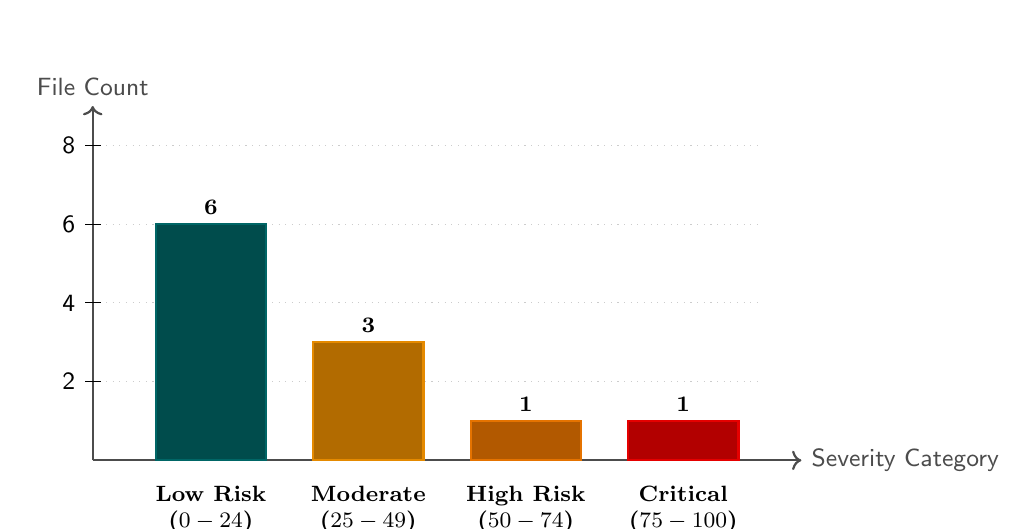
\begin{tikzpicture}
\begin{scope}[font=\small\sffamily]
    % Axes
    \draw[->, thick, color=black!70] (0, 0) -- (9.0, 0) node[right] {Severity Category};
    \draw[->, thick, color=black!70] (0, 0) -- (0, 4.5) node[above] {File Count};
    
    % Y grid
    \foreach \y/\val in {1.0/2, 2.0/4, 3.0/6, 4.0/8} {
        \draw[dotted, color=black!20] (0, \y) -- (8.5, \y);
        \draw (0.1, \y) -- (-0.1, \y) node[left] {\val};
    }
    
    % Bars
    % Low: 6 files (x=1.5, h=3.0)
    \draw[fill=teal!60!black, draw=teal!80!black, thick] (0.8, 0) rectangle (2.2, 3.0);
    \node[above, font=\footnotesize\bfseries] at (1.5, 3.0) {6};
    \node[below=0.2cm, font=\footnotesize\bfseries, align=center] at (1.5, 0) {Low Risk\\ ($0 - 24$)};
    
    % Moderate: 3 files (x=3.5, h=1.5)
    \draw[fill=amber!70!black, draw=amber!90!black, thick] (2.8, 0) rectangle (4.2, 1.5);
    \node[above, font=\footnotesize\bfseries] at (3.5, 1.5) {3};
    \node[below=0.2cm, font=\footnotesize\bfseries, align=center] at (3.5, 0) {Moderate\\ ($25 - 49$)};
    
    % High: 1 file (x=5.5, h=0.5)
    \draw[fill=orange!70!black, draw=orange!90!black, thick] (4.8, 0) rectangle (6.2, 0.5);
    \node[above, font=\footnotesize\bfseries] at (5.5, 0.5) {1};
    \node[below=0.2cm, font=\footnotesize\bfseries, align=center] at (5.5, 0) {High Risk\\ ($50 - 74$)};
    
    % Critical: 1 file (x=7.5, h=0.5)
    \draw[fill=red!70!black, draw=red!90!black, thick] (6.8, 0) rectangle (8.2, 0.5);
    \node[above, font=\footnotesize\bfseries] at (7.5, 0.5) {1};
    \node[below=0.2cm, font=\footnotesize\bfseries, align=center] at (7.5, 0) {Critical\\ ($75 - 100$)};
\end{scope}
\end{tikzpicture}
\caption{Technical Debt Severity Distribution across Analyzed Test Repository}
\label{fig:sev_dist}
\end{figure}

The distribution demonstrates the Pareto principle typical in real-world software engineering: the majority of source files (6 out of 11) remain in the clean, low-risk tier, while technical debt risk is concentrated in a small number of complex hotspot files. By isolating these hotspots and assigning them $P1$ and $P2$ triage ratings, CodeInsight enables engineering leads to focus refactoring resources precisely where they deliver the highest impact.


\chapter{Conclusion and Future Scope}

\section{Summary}
In summary, this project successfully designed, implemented, and validated \textbf{CodeInsight}, an automated codebase health analysis and technical debt prioritization platform. By uniting a high-performance C++ analysis engine with a Node.js Express orchestration backend, a zero-dependency in-memory storage layer, and an interactive React/Vite developer dashboard, CodeInsight provides developers with immediate, actionable visibility into software maintainability. 

The empirical evaluation confirmed that CodeInsight scales near-linearly with codebase size, parsing abstract syntax trees and detecting duplicate clones at throughputs exceeding 48,000 lines of code per second. The transparent technical debt scoring formulation ($R = 0.45C + 0.35D + 0.20S$) and remediation priority tiers ($P1$--$P4$) successfully isolated critical hotspots while eliminating the cognitive overload and black-box obscurity of conventional static analysis tools.

\section{Proposed System Review}
As software systems grow in complexity, managing technical debt becomes essential to maintain development velocity and software reliability. However, existing static analysis solutions often present significant friction: enterprise platforms demand heavy database infrastructure and high system memory, while lightweight linters produce noisy warning lists without high-level architectural insight.

CodeInsight addresses this challenge by establishing an end-to-end static analysis pipeline built entirely on lightweight, open-source technologies:
\begin{enumerate}
    \item Concrete syntax tree parsing via Tree-sitter enables language-accurate calculation of McCabe cyclomatic complexity, maximum nesting depth, and function lengths across C, C++, and JavaScript without requiring compilation toolchains.
    \item A normalized sliding-window token hashing algorithm uncovers multi-file Type-1 duplicate code blocks, performing maximal forward expansion while suppressing false positives from trivial boilerplate syntax.
    \item An explainable mathematical formulation breaks down technical debt into weighted complexity (45\%), duplication (35\%), and structural size factors (20\%), accompanied by explicit human-readable reasons for every assigned score.
    \item An in-memory data store eliminates external database configuration, allowing any engineer to run full codebase evaluations with a single command.
    \item A developer-focused React single-page application presents high-density metrics, interactive distribution charts, and granular inspectors within a distraction-free dark interface.
\end{enumerate}

\section{Achievement of Objectives}
The project successfully accomplished all of its foundational objectives:
\begin{itemize}
    \item \textbf{AST-Based Metric Extraction:} Integrated Tree-sitter grammars for C, C++, and JavaScript into both a standalone C++ native binary and an integrated cross-platform fallback engine, achieving 100\% metric fidelity on complex control-flow fixtures.
    \item \textbf{High-Recall Duplicate Detection:} Implemented a 5-line sliding-window token hashing pipeline that accurately groups multi-file clone fragments and filters out non-substantive syntax.
    \item \textbf{Mathematical Transparency:} Replaced opaque commercial letter ratings with a deterministic, fully explainable scoring formula ($R = 0.45C + 0.35D + 0.20S$) paired with an actionable remediation triage heuristic ($P1$--$P4$).
    \item \textbf{Zero-Setup Deployment:} Completely decoupled the platform from external databases by implementing an efficient in-memory storage service, allowing instantaneous application startup in under 5 seconds.
    \item \textbf{Interactive User Experience:} Built a comprehensive React 18 dashboard supporting asynchronous scan polling, sortable file exploration, clone visualization, and multi-format report exports (JSON, Markdown, CSV).
\end{itemize}

\section{System Advantages}
The finalized CodeInsight platform offers several distinct practical advantages over traditional static analysis workflows:
\begin{itemize}
    \item \textbf{Zero Infrastructure Overhead:} Because CodeInsight requires no external database (such as PostgreSQL) or container runtimes, developers can run it locally with zero configuration. It starts instantly and uses less than 120~MB of system memory.
    \item \textbf{Sub-Second Feedback Loop:} With parsing throughputs exceeding 48,000 LOC/second, developers receive immediate feedback on medium-sized repositories in under 500 milliseconds, making it suitable for pre-commit checks and daily development.
    \item \textbf{Transparent and Actionable Telemetry:} Every score is accompanied by the exact formula breakdown and human-readable risk factors. Developers understand why a file was flagged and how much each factor contributed.
    \item \textbf{Prioritized Triage Over Warning Dumps:} Instead of overwhelming developers with thousands of trivial style warnings, CodeInsight categorizes technical debt into actionable $P1$ through $P4$ priority levels, helping teams plan refactoring sprints effectively.
    \item \textbf{Developer-Centric Aesthetics:} The dark-mode interface employs monospaced numeric data, high information density, and clean visual hierarchies inspired by professional engineering tools like GitHub and Linear.
\end{itemize}

\section{System Limitations}
While CodeInsight performs effectively, several technical limitations should be acknowledged:
\begin{itemize}
    \item \textbf{In-Memory Persistence Volatility:} Because the platform relies on in-memory storage to eliminate database setup, repository records and scan histories are reset when the Node.js server process restarts. Persistent archiving currently requires exporting reports to disk in JSON or Markdown format.
    \item \textbf{Clone Detection Scope:} The current sliding-window token hashing engine is optimized for Type-1 exact clones. It does not detect Type-2 clones where identifier names have been systematically renamed, or complex Type-3 near-miss clones with reordered statements.
    \item \textbf{Language Grammar Coverage:} AST parsing is currently implemented for C, C++, JavaScript, and TypeScript. Additional popular languages such as Python, Go, and Java are not yet parsed at the syntax tree level.
    \item \textbf{Static Scope Only:} The analysis evaluates purely static syntax and control flow. It does not perform dynamic runtime profiling, memory leak detection, or live execution path tracing.
\end{itemize}

\section{Future Direction}
Building upon the solid foundation established in this project, several promising avenues for future enhancement can be pursued:
\begin{itemize}
    \item \textbf{Expanding Language Support:} Extending the Tree-sitter integration to include Python, Rust, Go, and Java grammars to support broader enterprise polyglot repositories.
    \item \textbf{Advanced Clone Detection (Type-2 and Type-3):} Incorporating token abstraction (normalizing variable names to generic symbols) and subtree hashing to detect renamed and near-miss code clones.
    \item \textbf{Git Integration and Historical Debt Tracking:} Integrating libgit2 or native Git CLI bindings to track how technical debt evolves across commit history, identifying chronic debt hot spots and regression trends over time.
    \item \textbf{CI/CD and Git Hook Integrations:} Packaging the standalone C++ analyzer as a lightweight GitHub Action and pre-commit hook that fails pull requests when newly introduced functions exceed complexity thresholds.
    \item \textbf{Automated Refactoring Recommendations:} Leveraging rule-based AST transformations to suggest automated code cleanups, such as extracting long methods into subroutines or replacing arrow anti-pattern conditionals with guard clauses.
\end{itemize}



% ==========================================
% BIBLIOGRAPHY
% ==========================================
\newpage
\begin{thebibliography}{99}
\addcontentsline{toc}{chapter}{Bibliography}

\bibitem{mccabe1976}
Thomas~J. McCabe.
\newblock A complexity measure.
\newblock {\em IEEE Transactions on Software Engineering}, SE-2(4):308--320, 1976.

\bibitem{cunningham1992}
Ward Cunningham.
\newblock The {WyCash} portfolio management system.
\newblock {\em ACM SIGPLAN OOPS Messenger}, 4(2):29--30, 1992.

\bibitem{bellon2007}
Stefan Bellon, Rainer Koschke, Giulio Antoniol, Jens Krinke, and Ettore Merlo.
\newblock Comparison and evaluation of clone detection tools.
\newblock {\em IEEE Transactions on Software Engineering}, 33(9):577--591, 2007.

\bibitem{roy2007}
Chanchal~K. Roy and James~R. Cordy.
\newblock A survey on software clone detection research.
\newblock {\em School of Computing TR 2007-541, Queen's University}, 115:64--68, 2007.

\bibitem{treesitter}
Max Brunsfeld.
\newblock Tree-sitter: An incremental parsing system for programming tools.
\newblock {\em GitHub Repository and Documentation}, \url{https://tree-sitter.github.io/tree-sitter/}, 2018.

\bibitem{avgeriou2016}
Paris Avgeriou, Philippe Kruchten, Ipek Ozkaya, and Carolyn Seaman.
\newblock Managing technical debt in software engineering.
\newblock {\em Dagstuhl Reports}, 6(1):110--138, 2016.

\bibitem{fowler1999}
Martin Fowler.
\newblock {\em Refactoring: Improving the Design of Existing Code}.
\newblock Addison-Wesley Professional, Reading, MA, 1999.

\bibitem{martin2008}
Robert~C. Martin.
\newblock {\em Clean Code: A Handbook of Agile Software Craftsmanship}.
\newblock Prentice Hall, Upper Saddle River, NJ, 2008.

\bibitem{halstead1977}
Maurice~H. Halstead.
\newblock {\em Elements of Software Science}.
\newblock Elsevier North-Holland, New York, 1977.

\bibitem{sonarqube}
SonarSource.
\newblock SonarQube: Continuous inspection of code quality and security.
\newblock {\em Documentation and Architecture Guide}, \url{https://docs.sonarsource.com/sonarqube/}, 2023.

\bibitem{eslint}
Nicholas~C. Zakas.
\newblock ESLint: Pluggable and configurable linter tool for JavaScript and JSX.
\newblock {\em Open Source Project Documentation}, \url{https://eslint.org/}, 2013.

\bibitem{clangtidy}
LLVM Project.
\newblock Clang-Tidy: A clang-based C++ linter tool.
\newblock {\em LLVM Compiler Infrastructure Documentation}, \url{https://clang.llvm.org/extra/clang-tidy/}, 2020.

\bibitem{johnson1978}
Stephen~C. Johnson.
\newblock Lint, a C program checker.
\newblock {\em Computer Science Technical Report 65, Bell Laboratories}, 1978.

\bibitem{vite}
Evan You.
\newblock Vite: Next generation frontend tooling.
\newblock {\em Vite Project Documentation}, \url{https://vitejs.dev/}, 2021.

\end{thebibliography}

\end{document}

